\documentclass{ctexart}
\setmainfont{Times New Roman}
\usepackage{amsmath}
\usepackage{amsfonts,amsmath,amsthm}
\usepackage{amssymb}
\usepackage{mathrsfs}
\usepackage{bbm}
\usepackage{fancyhdr}
\usepackage[a4paper,left=2.5cm,right=2.5cm,top=2cm,bottom=2cm]{geometry}
\usepackage[linkcolor=black,citecolor=black,colorlinks=true,linkcolor=black,citecolor=black,urlcolor=black]{hyperref}
\usepackage{color}
\usepackage{tikz}
\usetikzlibrary{arrows.meta}
\usepackage{diagbox}
\usepackage{multicol}
\usepackage{arydshln}
\usepackage{xparse}
\usepackage{pgfplots}
\usepackage{comment}
\usepackage{graphicx}
\usepackage{bm}
\usetikzlibrary{angles, calc}
\usetikzlibrary{positioning, shapes.geometric}
\usetikzlibrary{graphs}
\usepackage{fancyhdr}
\lhead{\today}
\rhead{}
\cfoot{}

\usepackage{pdfpages}
\usepackage{tabu}
\usepackage{threeparttable}
\usepackage{listings}
\usepackage{paralist}
\usepackage{appendix}
\usepackage{lastpage}
\usepackage{longtable,multirow,array}
\usepackage{booktabs}
\usepackage{tabularx}
\usepackage{xstring}
\usepackage{tipa}
\usepackage[framemethod=TikZ]{mdframed}
\mdfdefinestyle{extrastyle}{%
    linecolor=gray,
    linewidth=1pt,
    frametitlerule=true,
    frametitlebackgroundcolor=gray!10,
    backgroundcolor=gray!5,
    skipabove=10pt,
    skipbelow=10pt,
    innertopmargin=5pt,
    innerbottommargin=5pt
}
\newenvironment{extra}{\begin{mdframed}[style=extrastyle, frametitle={* 选读内容（不要求掌握）}]}{\end{mdframed}}

\newcommand{\upcite}[1]{\textsuperscript{\textsuperscript{\cite{#1}}}}
\newcommand{\bec}{\kern 0.56em\bigcirc \kern -0.85em {\small \because}\kern 0.56em}
\DeclareMathOperator*{\argmax}{\mathrm{arg\,max}}
\DeclareMathOperator*{\argmin}{\mathrm{arg\,min}}
\newcounter{EnvironmentCounter}
% ==================== 环境计数器定义 ====================
% 为每种环境单独定义计数器，使其独立编号
\newcounter{problemCounter}
\newcounter{theoremCounter}
\newcounter{conclusionCounter}
\newcounter{definitionCounter}
\newcounter{exampleCounter}
\newcounter{propositionCounter}
\newcounter{exerciseCounter}

% ==================== 问题环境 ====================
\NewDocumentEnvironment{problem}{O{}}
{
    \par\noindent 
    \refstepcounter{problemCounter}
    \textbf{问题 \theproblemCounter\IfNoValueOrEmpty{#1}{}{ (#1)}}\quad
}
{
    \par\vspace{1em}
}

% ==================== 定理环境 ====================
\NewDocumentEnvironment{theorem}{O{}}
{
    \par\noindent 
    \refstepcounter{theoremCounter}
    \textbf{定理 \thetheoremCounter\IfNoValueOrEmpty{#1}{}{ (#1)}}\quad
}
{
    \par\vspace{1em}
}

% ==================== 结论环境 ====================
\NewDocumentEnvironment{conclusion}{O{}}
{
    \par\noindent 
    \refstepcounter{conclusionCounter}
    \textbf{结论 \theconclusionCounter\IfNoValueOrEmpty{#1}{}{ (#1)}}\quad
}
{
    \par\vspace{1em}
}

% ==================== 定义环境 ====================
\NewDocumentEnvironment{definition}{O{}}
{
    \par\noindent 
    \refstepcounter{definitionCounter}
    \textbf{定义 \thedefinitionCounter\IfNoValueOrEmpty{#1}{}{ (#1)}}\quad
}
{
    \par\vspace{1em}
}

% ==================== 例环境 ====================
\NewDocumentEnvironment{example}{O{}}
{
    \par\noindent 
    \refstepcounter{exampleCounter}
    \textbf{例 \theexampleCounter\IfNoValueOrEmpty{#1}{}{}}\quad
}
{
    \par\vspace{1em}
}

% ==================== 性质环境 ====================
\NewDocumentEnvironment{proposition}{O{}}
{
    \par\noindent 
    \refstepcounter{propositionCounter}
    \textbf{性质 \thepropositionCounter\IfNoValueOrEmpty{#1}{}{ (#1)}}\quad
}
{
    \par\vspace{1em}
}

% ==================== 练习环境 ====================
\NewDocumentEnvironment{exercise}{O{}}
{
    \par\noindent 
    \refstepcounter{exerciseCounter}
    \textbf{练习 \theexerciseCounter\IfNoValueOrEmpty{#1}{}{ }}\quad
}
{
    \par\vspace{1em}
}

% ==================== 辅助命令 ====================
% 如果需要重置某个计数器，可使用以下命令
\newcommand{\resetProblemCounter}{\setcounter{problemCounter}{0}}
\newcommand{\resetTheoremCounter}{\setcounter{theoremCounter}{0}}
\newcommand{\resetConclusionCounter}{\setcounter{conclusionCounter}{0}}
\newcommand{\resetDefinitionCounter}{\setcounter{definitionCounter}{0}}
\newcommand{\resetExampleCounter}{\setcounter{exampleCounter}{0}}
\newcommand{\resetPropositionCounter}{\setcounter{propositionCounter}{0}}
\newcommand{\resetExerciseCounter}{\setcounter{exerciseCounter}{0}}

% 如需一次性重置所有计数器
\newcommand{\resetAllCounters}{%
    \resetProblemCounter%
    \resetTheoremCounter%
    \resetConclusionCounter%
    \resetDefinitionCounter%
    \resetExampleCounter%
    \resetPropositionCounter%
    \resetExerciseCounter%
}
\newcommand{\renewEnvironmentCounter}{\setcounter{EnvironmentCounter}{0}}
\newcommand{\dd}{\mathrm{d}}
\renewcommand{\textfraction}{0.15}
\renewcommand{\topfraction}{0.85}
\renewcommand{\bottomfraction}{0.65}
\renewcommand{\floatpagefraction}{0.60}
\renewcommand{\figurename}{图}
\renewcommand{\tablename}{表}
\setlength{\belowcaptionskip}{4pt}
\setlength{\abovecaptionskip}{4pt}
\newenvironment{custom}[1]{\par\noindent \textbf{#1}\quad}{\par\vspace{1em}}
\lstset{
  language=Matlab,
  basicstyle=\ttfamily\small,
  breaklines=true,
  keywordstyle=\color{blue},
  commentstyle=\color[rgb]{0.13,0.55,0.13},
  stringstyle=\color[rgb]{0.7,0.15,0.15},
  numbers=left,
  stepnumber=1,
  showstringspaces=false
}
\lstset{
    tabsize=4,
    breaklines=true,
    basicstyle=\ttfamily,
}
\title{大学数学I 讲义（第1-4周）}
\author{}
\date{}
\graphicspath{{plot/}}
\let\itemize\compactitem
\let\enditemize\endcompactitem
\DeclareGraphicsExtensions{.pdf, .jpg, .tif, .png}
\tikzset{every picture/.style={line width=0.75pt}}
\begin{document}
\maketitle
\rhead{Page \thepage\ of \pageref{LastPage}}
\renewcommand{\contentsname}{\hspace*{\fill}\Large\bfseries 目\quad 录 \hspace*{\fill}}
\setcounter{tocdepth}{2}
\tableofcontents 
\clearpage
\pagestyle{fancy}

\section{数列的基本概念}

\subsection{从高中数列说起}

在高中数学中，我们已经接触过两种重要的数列。

\begin{example}[等差数列]


\textbf{故事引入：} 相传数学家高斯在小学时，老师让同学们计算 \(1 + 2 + \cdots + 100\)。当其他同学还在埋头苦算时，小高斯很快给出了答案 5050。他发现：
\[
1+100=101,\ 2+99=101,\ \cdots,\ 50+51=101,
\]
共 50 对，所以总和是 \(50 \times 101 = 5050\)。这个数列 \(1,2,3,\dots\) 就是等差数列。

\textbf{定义：} 从第二项起，每一项与前一项的差是同一个常数 \(d\)，即
\[
a_{n+1} - a_n = d \quad (\text{常数}).
\]
通项公式：\(a_n = a_1 + (n-1)d\)。例如：\(1,3,5,7,\dots\)（\(d=2\)）。
\end{example}

\begin{example}[等比数列]


\textbf{故事引入：} 传说国际象棋的发明者向国王要麦子：第一个格子放 1 粒，第二个放 2 粒，第三个放 4 粒，以此类推，每个格子放前一个的两倍。国王以为这很容易，结果发现整个国家的粮食都不够。这个数列 \(1,2,4,8,\dots\) 就是等比数列。

\textbf{定义：} 从第二项起，每一项与前一项的比是同一个常数 \(r\)，即
\[
\dfrac{a_{n+1}}{a_n} = r \quad (\text{常数}).
\]
通项公式：\(a_n = a_1 r^{n-1}\)。例如：\(1,\dfrac12,\dfrac14,\dfrac18,\dots\)（\(r=\dfrac12\)）。
\end{example}

\subsection{数列的一般定义}

将高中学过的数列概念推广，我们得到数列的一般定义。

\begin{definition}[数列]
按一定次序排列的一列数称为数列，记为 \(\{a_n\}\)。其中 \(a_n\) 称为通项，\(n\) 称为下标。
\end{definition}

数列本质上是一个从正整数集 \(\mathbb{N}^*\) 到实数集 \(\mathbb{R}\) 的映射：
\[
a_n = f(n),\quad n=1,2,3,\dots
\]
数列就是“一列按顺序排好的数”。你可以想象成一条无限长的队伍，每个人都戴着一个号码牌，上面写着一个数。这个号码牌上的数，就是数列的“第 n 项”。

\subsection{数列的几种其他定义方式}

\begin{custom}{方式一：列出前几项}
例如：\(1, \dfrac12, \dfrac13, \dfrac14, \dots\)，猜想通项为 \(a_n = \dfrac1n\)。

注意：这种定义方式不严格，因为前几项可能对应多种通项。例如 \(1,2,4,\dots\) 可以是 \(a_n=2^{n-1}\)，也可以是 \(a_n = \dfrac{n^2-n+2}{2}\)。
\end{custom}

\begin{custom}{方式二：通项公式}
直接给出 \(a_n = \dfrac{n+1}{2n-1}\)，则可算出任意一项。这是最常用的定义方式。
\end{custom}

\begin{custom}{方式三：递推关系}
用前面项表示后面项。例如：
\[
a_1 = 1,\ a_2 = 1,\ a_n = a_{n-1} + a_{n-2}\ (n \geq 3),
\]
这就是著名的\textbf{斐波那契数列}：\(1,1,2,3,5,8,13,21,\dots\)

自然界中很多现象与斐波那契数列有关：向日葵的种子排列（常出现 34,55,89 等斐波那契数）、鹦鹉螺的螺旋线、甚至兔子繁殖问题。
\end{custom}

\subsection{数列在生活与生产中的应用}

数列不仅仅是课本上的抽象概念，它在我们的日常生活和现代生产中有着广泛的应用。下面介绍几个有趣的实例。

\begin{custom}{应用一：算法分析与计算机科学}

在计算机科学中，算法的\textbf{时间复杂度}经常用数列来描述。例如，考虑一个在有序数组中查找元素的算法：

\begin{itemize}
\item \textbf{二分查找}：每次将搜索范围缩小一半。在最坏情况下，需要查找的次数满足递推关系：
\[
T(n) = T\left(\dfrac{n}{2}\right) + 1,\quad T(1) = 1.
\]
解这个递推，得到 \(T(n) = \lceil \log_2 n \rceil\)。这是一个对数增长数列——非常高效！


一个著名的例子是\textbf{汉诺塔}问题：把 \(n\) 个圆盘从一根柱子移到另一根，最少需要移动的次数满足：
\[
H_n = 2H_{n-1} + 1,\quad H_1 = 1.
\]
解这个递推得 \(H_n = 2^n - 1\)——指数增长！64 个圆盘需要移动 \(2^{64}-1\) 次，即使每秒移动一次，也需要约 5849 亿年。
\end{custom}

\begin{custom}{应用二：自然界中的斐波那契数列}

斐波那契数列 \(1, 1, 2, 3, 5, 8, 13, 21, 34, 55, \ldots\) 在自然界中随处可见：

\begin{itemize}
\item \textbf{向日葵的花盘}：种子排列成两组螺旋线，一组顺时针，一组逆时针，数量通常是相邻的斐波那契数（如 34 和 55，或 55 和 89）。
\item \textbf{松果的鳞片}：排列也呈现斐波那契螺旋。
\item \textbf{鹦鹉螺的壳}：其对数螺线的生长比例接近黄金分割比 \(\varphi \approx 1.618\)，而 \(\varphi\) 与斐波那契数列密切相关（\(\lim_{n\to\infty} \dfrac{F_{n+1}}{F_n} = \varphi\)）。
\item \textbf{蜜蜂的家族树}：雄蜂（由未受精卵发育而来）的祖先数量构成斐波那契数列。
\item \textbf{花瓣数}：许多花的花瓣数是 3（百合）、5（飞燕草）、8（翠雀）、13（金盏花）、21（紫菀）等斐波那契数。
\end{itemize}

\begin{center}
\begin{tikzpicture}
% 简单的向日葵螺旋示意图
\foreach \i in {1,...,50} {
    \pgfmathsetmacro{\r}{0.3*sqrt(\i)}
    \pgfmathsetmacro{\theta}{137.5*\i}
    \filldraw[orange] (\theta:\r) circle (1.5pt);
}
\node at (0, -3) {向日葵种子的螺旋排列（示意图）};
\end{tikzpicture}
\end{center}

大自然为什么“偏爱”斐波那契数？科学家认为，这种排列方式可以让种子最紧密地堆积，充分利用空间——这是自然选择的结果，也是数学与生命的美妙交汇。
\end{custom}

\begin{custom}{应用三：工程中的递归设计与分形}

在工程和建筑设计领域，许多结构采用\textbf{自相似}的设计——即整体与局部形状相似。这种递归结构可以用数列来描述。

\begin{itemize}
\item \textbf{分形天线}：手机天线采用分形设计，可以在有限空间内获得更长的有效长度，从而接收更多频段的信号。
\item \textbf{谢尔宾斯基三角形}：一个不断“挖空”的三角形图案，它的面积随迭代次数构成一个等比数列：\(A_n = \left(\dfrac{3}{4}\right)^n A_0\)。
\item \textbf{科赫雪花}：一条不断“加尖”的曲线，它的周长随迭代次数无限增长（\(L_n = \left(\dfrac{4}{3}\right)^n L_0\)），但面积却收敛到有限值。
\end{itemize}

这些例子展示了：数列不仅是描述离散过程的工具，还连接着几何、物理和工程。
\end{custom}

\subsection{差分及其应用}

在微积分中，我们通过导数研究函数的变化率。对于数列，差分扮演着类似的角色。

\begin{definition}[差分]
对于数列 \(\{a_n\}\)，定义：
\begin{itemize}
\item 一阶差分：\(\Delta a_n = a_{n+1} - a_n\)；
\item 二阶差分：\(\Delta^2 a_n = \Delta(\Delta a_n) = a_{n+2} - 2a_{n+1} + a_n\)；
\item \(k\) 阶差分：\(\Delta^k a_n = \Delta(\Delta^{k-1} a_n)\)。
\end{itemize}
\end{definition}

\begin{proposition}[差分的性质]
\begin{enumerate}
\item \(\Delta C = 0\)（\(C\) 为常数）；
\item \(\Delta(C a_n) = C \Delta a_n\)；
\item \(\Delta(a_n + b_n) = \Delta a_n + \Delta b_n\)。
\end{enumerate}
\end{proposition}

差分的一个核心应用是数列求和。

\begin{theorem}[离散牛顿-莱布尼茨公式]
\[
\sum_{k=m}^{n-1} \Delta a_k = a_n - a_m.
\]
特别地，\(\sum_{k=1}^{n-1} \Delta a_k = a_n - a_1\)。
\end{theorem}

这个公式告诉我们：如果能找到一个数列 \(b_k\) 使得 \(\Delta b_k = a_k\)，那么 \(\sum a_k = b_n - b_1\)。这正是“差分是求和的逆运算”。

\begin{example}[求自然数平方和]
求 \(\sum_{k=1}^n k^2\)。
\end{example}

\begin{custom}{解}
观察发现 \(\Delta k^3 = (k+1)^3 - k^3 = 3k^2 + 3k + 1\)，所以
\[
3\sum_{k=1}^n k^2 = \sum_{k=1}^n \Delta k^3 - 3\sum_{k=1}^n k - \sum_{k=1}^n 1.
\]
利用 \(\sum k = \dfrac{n(n+1)}{2}\) 和 \(\sum 1 = n\)，以及 \(\sum \Delta k^3 = (n+1)^3 - 1\)，可得
\[
3\sum k^2 = (n+1)^3 - 1 - \dfrac{3n(n+1)}{2} - n = \dfrac{n(n+1)(2n+1)}{2},
\]
所以 \(\sum_{k=1}^n k^2 = \dfrac{n(n+1)(2n+1)}{6}\)。
\end{custom}

\begin{example}[进阶：求 \(\sum_{k=1}^n k^2 \cdot 2^k\)]
这类“多项式乘指数”的求和，可以用待定系数法构造差分。
\end{example}

\begin{custom}{解}
设 \(b_k = (Ak^2 + Bk + C)2^k\)，目标是使 \(\Delta b_k = k^2 2^k\)。
计算 \(\Delta b_k = b_{k+1} - b_k = [A(k+1)^2 + B(k+1) + C]2^{k+1} - (Ak^2 + Bk + C)2^k = 2^k[2A(k+1)^2 + 2B(k+1) + 2C - (Ak^2 + Bk + C)]\)。
整理得 \(\Delta b_k = 2^k[Ak^2 + (4A + B)k + (2A + 2B + C)]\)。
令其等于 \(k^2 2^k\)，比较系数：
\[
\begin{cases}
A = 1,\\
4A + B = 0,\\
2A + 2B + C = 0.
\end{cases}
\]
解得 \(A=1,\ B=-4,\ C=6\)，即 \(b_k = (k^2 - 4k + 6)2^k\)。
于是
\[
\sum_{k=1}^n k^2 2^k = \sum_{k=1}^n \Delta b_k = b_{n+1} - b_1 = [(n+1)^2 - 4(n+1) + 6]2^{n+1} - (1-4+6)\cdot 2 = (n^2 - 2n + 3)2^{n+1} - 6.
\]
\end{custom}

\subsection*{练习题：数列的定义、递推关系与差分}

\begin{exercise}写出下列数列的通项公式 \(a_n\)（用 \(n\) 表示）：
\begin{enumerate}
\item \(1, 3, 5, 7, 9, \dots\)
\item \(2, 4, 8, 16, 32, \dots\)
\item \(\dfrac{1}{2}, \dfrac{2}{3}, \dfrac{3}{4}, \dfrac{4}{5}, \dfrac{5}{6}, \dots\)
\item \(1, -\dfrac{1}{2}, \dfrac{1}{3}, -\dfrac{1}{4}, \dfrac{1}{5}, \dots\)
\end{enumerate}
\end{exercise}

\begin{exercise}已知下列递推关系及初始条件，写出数列的前 5 项：
\begin{enumerate}
\item \(a_1 = 3\)，\(a_n = 2a_{n-1}\)（\(n \geq 2\)）
\item \(a_1 = 1\)，\(a_n = a_{n-1} + n\)（\(n \geq 2\)）
\item \(a_1 = 1\)，\(a_2 = 3\)，\(a_n = a_{n-1} - a_{n-2}\)（\(n \geq 3\)）
\end{enumerate}
\end{exercise}

\begin{exercise}对于数列 \(a_n = n^2\)，计算：
\begin{enumerate}
\item 一阶差分 \(\Delta a_n\)
\item 二阶差分 \(\Delta^2 a_n\)
\item 三阶差分 \(\Delta^3 a_n\)
\end{enumerate}
观察结果，你能发现什么规律？
\end{exercise}

\begin{exercise}求下列递推数列的通项公式：
\begin{enumerate}
\item \(a_1 = 1\)，\(a_n = a_{n-1} + 3\)（\(n \geq 2\)）
\item \(a_1 = 5\)，\(a_n = a_{n-1} + 2n - 1\)（\(n \geq 2\)）
\item \(a_1 = 2\)，\(a_n = 2a_{n-1} + 1\)（\(n \geq 2\)）\quad（提示：可设 \(b_n = a_n + 1\) 构造等比数列）
\end{enumerate}
\end{exercise}

\begin{exercise}求一个数列 \(b_n\)，使得 \(\Delta b_n = n \cdot 2^n\)。
提示：设 \(b_n = (An + B)2^n\)，代入确定系数 \(A, B\)。
\end{exercise}

\begin{exercise}用差分法求下列和式：
\begin{enumerate}
\item \(\sum_{k=1}^{n} k\)
\item \(\sum_{k=1}^{n} k(k+1)\)
\end{enumerate}
\end{exercise}

\begin{exercise}已知斐波那契数列：\(F_1 = 1, F_2 = 1, F_n = F_{n-1} + F_{n-2} (n \geq 3)\)。
\begin{enumerate}
\item 计算比值 \(\dfrac{F_6}{F_5}, \dfrac{F_7}{F_6}, \dfrac{F_8}{F_7}, \dfrac{F_9}{F_8}, \dfrac{F_{10}}{F_9}\)，观察它们趋近于哪个数。
\item 证明：\(F_{n+1}F_{n-1} - F_n^2 = (-1)^n\)（卡西尼恒等式）。（选做）
\end{enumerate}
\end{exercise}

\begin{exercise}已知数列 \(\{a_n\}\) 满足 \(a_1 = 1\)，且对任意 \(n \geq 1\) 有 \(\Delta a_n = 3^n\)。
\begin{enumerate}
\item 求 \(a_n\) 的通项公式。
\item 计算 \(\sum_{k=1}^{n} k \cdot 3^{k-1}\)。（提示：利用 \(a_n\) 的表达式）
\end{enumerate}
\end{exercise}

\begin{exercise}已知一个数列的前几项为：\(a_1 = 1, a_2 = 5, a_3 = 14, a_4 = 30, a_5 = 55\)。
\begin{enumerate}
\item 计算该数列的一阶、二阶、三阶差分。
\item 根据差分结果判断 \(a_n\) 可能是几次多项式。
\item 求出 \(a_n\) 的通项公式。
\end{enumerate}
\end{exercise}

\begin{exercise}[较难：递推与差分的综合应用]
设数列 \(\{a_n\}\) 满足 \(a_1 = 1\)，且 \(a_{n+1} = 3a_n + 2^n\)（\(n \geq 1\)）。
\begin{enumerate}
\item 令 \(b_n = \dfrac{a_n}{2^n}\)，写出 \(b_n\) 满足的递推关系。
\item 求 \(b_n\) 的通项公式。
\item 求 \(a_n\) 的通项公式。
\item 计算 \(\sum_{k=1}^{n} a_k\)。
\end{enumerate}
\end{exercise}

\newpage 

\begin{custom}{参考答案提要}

\begin{enumerate}
\item[(1)] (a) \(a_n = 2n-1\)；(b) \(a_n = 2^n\)；(c) \(a_n = \dfrac{n}{n+1}\)；(d) \(a_n = (-1)^{n-1} \dfrac{1}{n}\)。
\item[(2)] (a) \(3, 6, 12, 24, 48\)；(b) \(1, 3, 6, 10, 15\)；(c) \(1, 3, 2, -1, -3\)。
\item[(3)] \(\Delta a_n = 2n+1\)，\(\Delta^2 a_n = 2\)，\(\Delta^3 a_n = 0\)；规律：\(n^2\) 的二阶差分为常数，三阶及更高阶为 0。
\item[(4)] (a) \(a_n = 3n-2\)；(b) \(a_n = n^2 + 4\)；(c) \(a_n = 2^{n+1} - 1\)。
\item[(5)] \(b_n = (n-2)2^{n-1} + C\)（\(C\) 为任意常数）。
\item[(6)] (a) \(\dfrac{n(n+1)}{2}\)；(b) \(\dfrac{n(n+1)(n+2)}{3}\)。
\item[(7)] 比值趋近于 \(\dfrac{1+\sqrt{5}}{2} \approx 1.618\)。
\item[(8)] (a) \(a_n = \dfrac{3^n - 1}{2}\)；(b) \(\sum_{k=1}^{n} k \cdot 3^{k-1} = \dfrac{(2n-1)3^n + 1}{4}\)。
\item[(9)] 三阶差分为常数 3，是三次多项式，\(a_n = \dfrac{n^3 + 5n}{6}\)。
\item[(10)] (a) \(b_{n+1} = \dfrac{3}{2} b_n + \dfrac{1}{2}\)；(b) \(b_n = 3\left(\dfrac{3}{2}\right)^{n-1} - 1\)；(c) \(a_n = 3^n - 2^n\)；(d) \(\sum_{k=1}^{n} a_k = \dfrac{3^{n+1} - 3}{2} - (2^{n+1} - 2)\)。
\end{enumerate}
\end{custom}

\clearpage
\section{数列极限}

\subsection{从实数的完备性说起}

\textbf{一个历史故事：} 古希腊的毕达哥拉斯学派信奉“万物皆数”，认为一切量都可以表示为整数的比（即有理数）。然而，该学派成员希帕索斯发现，边长为 1 的正方形的对角线长度 \(\sqrt{2}\) 不能表示为两个整数的比。这个发现震惊了整个学派，希帕索斯因此被投入大海。

这个故事告诉我们：有理数是不够用的。数轴上还有很多“空隙”——无理数。

\subsection{实数的构造与完备性}

\begin{custom}{有理数的局限}
有理数可以写成 \(\dfrac{p}{q}\)（\(p,q\) 为整数，\(q \neq 0\)）。但 \(\sqrt{2}\) 呢？

假设 \(\sqrt{2} = \dfrac{p}{q}\)（最简分数），则 \(2q^2 = p^2\)。左边有奇数个因子 2，右边有偶数个，矛盾！所以 \(\sqrt{2}\) 不是有理数。
\end{custom}

\begin{custom}{有理数稠密但不完备}
有理数在数轴上是“稠密”的：任意两个有理数之间总存在另一个有理数。但数轴上仍然有“空隙”——无理数。

例如，考虑有理数数列：
\[
1.4,\ 1.41,\ 1.414,\ 1.4142,\ 1.41421,\ \dots
\]
这些数都是有理数（有限小数），它们越来越接近 \(\sqrt{2}\)。但这个数列的“极限”\(\sqrt{2}\) 却不在有理数集中！
\end{custom}

\begin{custom}{实数的完备性}
实数系的一个重要性质是：任何收敛的实数数列，其极限仍然是实数。这称为实数的\textbf{完备性}（或连续性）。正是这个性质，使得极限理论得以建立。

简单来说：实数集对极限运算是“封闭”的——做极限操作不会跑出实数集。
\end{custom}

\subsection{数列极限的直观理解}

考虑数列 \(a_n = \dfrac{1}{n}\)：
\[
a_1=1,\ a_2=0.5,\ a_3\approx 0.333,\ a_{10}=0.1,\ a_{100}=0.01,\ a_{1000}=0.001.
\]
当 \(n\) 越来越大时，\(a_n\) 越来越接近 0。

问题是：如何用数学语言精确描述“越来越接近”？

\subsection{\(\varepsilon\)-\(N\) 定义}

\begin{definition}[数列极限]
设 \(\{a_n\}\) 为数列，\(A\) 为常数。如果对任意给定的 \(\varepsilon > 0\)，总存在正整数 \(N\)，使得当 \(n > N\) 时，有
\[
|a_n - A| < \varepsilon,
\]
则称数列 \(\{a_n\}\) 收敛于 \(A\)，记作 \(\lim\limits_{n\to\infty} a_n = A\)。
\end{definition}

\textbf{理解这个定义：}
\begin{itemize}
\item \(\varepsilon\) 代表“精度要求”——你想要多接近？
\item \(N\) 代表“从哪一项开始”——你需要等多久？
\item 定义说：无论你提出多高的精度要求（\(\varepsilon\) 多小），我总能找到一个 \(N\)，使得从第 \(N+1\) 项开始，所有项都与 \(A\) 的差距小于这个精度。
\end{itemize}

\subsection{数列极限的几个注解}

初学者对极限概念常有误解。下面几个注记可以帮助你更准确地理解“极限”这个词的真正含义。

\subsubsection{注一：没有一项等于极限值，也可以有极限}

很多人以为，既然极限是 \(a_n\) 趋向的那个数，那么到了某个很大的 \(n\)，\(a_n\) 就一定会等于极限值。这是不对的。

考虑数列 \(a_n = \dfrac{1}{n}\)。它的极限是 0，但你能找到一项 \(\dfrac{1}{n}\) 真正等于 0 吗？不能。不管 \(n\) 多大，\(\dfrac{1}{n}\) 永远是正数，只是越来越接近 0，但永远到不了 0。

再看数列 \(a_n = \dfrac{(-1)^n}{n}\)。它的极限也是 0，但有些项是正的（当 \(n\) 为偶数），有些项是负的（当 \(n\) 为奇数），没有一项是 0。

\textbf{结论：} 极限描述的是数列的“趋势”或“归宿”，而不是要求某项恰好等于它。就像一个不断靠近终点的人，他可以永远不踩到终点线，但我们仍然可以说他在趋近终点。

\subsubsection{注二：趋向极限的过程不一定单调，可以“左摇右摆”}

你可能从 \(\dfrac{1}{n}\) 这个例子中产生了错觉，以为数列趋近极限时应该越来越近，一路不回头。实际上不是这样。

考虑数列 \(a_n = \dfrac{(-1)^n}{n}\)：
\[
a_1 = -1,\ a_2 = 0.5,\ a_3 \approx -0.333,\ a_4 = 0.25,\ a_5 = -0.2,\ a_6 \approx 0.167,\ \dots
\]
它一会儿正，一会儿负，像醉汉走路一样左右摇晃。但摇晃的幅度越来越小——从 1 到 0.5 到 0.333 到 0.25……最终还是被“吸”向 0。

再比如 \(a_n = \dfrac{\sin n}{n}\)，它在 0 附近上下波动，但波动越来越微弱。

\textbf{结论：} 极限不要求数列单调。数列可以曲折、振荡、来回跳跃，只要最终“摇晃的幅度”趋于零，它仍然收敛。

\subsubsection{注三：等价于“极限点附近任意小的圆内，都有无穷多项”}

极限的严格定义是 \(\varepsilon\)-\(N\) 语言，但我们可以换一种更直观的说法：

\emph{如果 \(L\) 是数列的极限，那么无论你画一个多么小的圆（以 \(L\) 为中心，半径 \(\varepsilon > 0\)），这个圆内都含有数列的无穷多项（实际上是从某一项以后的所有项）。}

反过来，如果某个点附近的小圆内只含有有限多项（比如只有前几项在里面），那这个点就不是极限。

这个比喻可以帮助你直观判断：极限就是数列最终“扎堆”聚集的地方。就像一群鸟最终都落在一根树枝上——你可以选一个很小的范围，最终所有的鸟都在这个范围里。

\subsection{用定义证明极限}

\begin{example}
证明 \(\lim\limits_{n\to\infty} \dfrac{1}{n} = 0\)。
\end{example}
\begin{custom}{证}
对任意 \(\varepsilon > 0\)，要使 \(\left|\dfrac{1}{n} - 0\right| = \dfrac{1}{n} < \varepsilon\)，只需 \(n > \dfrac{1}{\varepsilon}\)。
取 \(N = \left\lceil \dfrac{1}{\varepsilon} \right\rceil\)，则当 \(n > N\) 时，有 \(\dfrac{1}{n} < \varepsilon\)。故极限为 0。\(\square\)
\end{custom}

\begin{example}
证明 \(\lim\limits_{n\to\infty} \dfrac{2n+1}{3n-2} = \dfrac{2}{3}\)。
\end{example}
\begin{custom}{证}
\[
\left|\dfrac{2n+1}{3n-2} - \dfrac{2}{3}\right| = \left|\dfrac{3(2n+1)-2(3n-2)}{3(3n-2)}\right| = \dfrac{7}{3(3n-2)}.
\]
对 \(\varepsilon > 0\)，要使 \(\dfrac{7}{3(3n-2)} < \varepsilon\)，只需 \(3n-2 > \dfrac{7}{3\varepsilon}\)，即 \(n > \dfrac{7}{9\varepsilon} + \dfrac{2}{3}\)。
取 \(N = \left\lceil \dfrac{7}{9\varepsilon} + \dfrac{2}{3} \right\rceil\)，则当 \(n > N\) 时不等式成立。\(\square\)
\end{custom}

\begin{example}
证明 \(\lim\limits_{n\to\infty} \left(\sqrt{n+1} - \sqrt{n}\right) = 0\)。
\end{example}
\begin{custom}{证}
先进行分子有理化：
\[
\left|\sqrt{n+1} - \sqrt{n} - 0\right| = \dfrac{(\sqrt{n+1} - \sqrt{n})(\sqrt{n+1} + \sqrt{n})}{\sqrt{n+1} + \sqrt{n}} = \dfrac{1}{\sqrt{n+1} + \sqrt{n}} < \dfrac{1}{2\sqrt{n}}.
\]
对任意 \(\varepsilon > 0\)，要使 \(\dfrac{1}{2\sqrt{n}} < \varepsilon\)，只需 \(\sqrt{n} > \dfrac{1}{2\varepsilon}\)，即 \(n > \dfrac{1}{4\varepsilon^2}\)。
取 \(N = \left\lceil \dfrac{1}{4\varepsilon^2} \right\rceil\)，则当 \(n > N\) 时，有 \(\left|\sqrt{n+1} - \sqrt{n}\right| < \varepsilon\)。故极限为 0。\(\square\)
\end{custom}

\begin{custom}{注}
这个例子说明：当直接处理表达式困难时，可以通过分子有理化、放缩等技巧转化为容易处理的形式。
\end{custom}

\begin{example}
证明 \(\lim\limits_{n\to\infty} \dfrac{n \sin n}{n^2 + 1} = 0\)。
\end{example}
\begin{custom}{证}
注意到 \(|\sin n| \leq 1\)，因此
\[
\left|\dfrac{n \sin n}{n^2 + 1} - 0\right| = \dfrac{n |\sin n|}{n^2 + 1} \leq \dfrac{n}{n^2 + 1} < \dfrac{n}{n^2} = \dfrac{1}{n}.
\]
对任意 \(\varepsilon > 0\)，取 \(N = \left\lceil \dfrac{1}{\varepsilon} \right\rceil\)，则当 \(n > N\) 时，有
\[
\left|\dfrac{n \sin n}{n^2 + 1}\right| \leq \dfrac{1}{n} < \varepsilon.
\]
故极限为 0。\(\square\)
\end{custom}

\begin{custom}{注}
这个例子展示了“放缩法”的核心思想：将复杂的表达式放大成一个简单形式（如 \(\dfrac{1}{n}\)），再对简单形式估计 \(N\)。这里的关键是 \(|\sin n| \leq 1\) 这个有界性。
\end{custom}

\begin{example}证明 \(\lim\limits_{n\to\infty} \dfrac{3n^2 + 2n - 1}{n^2 + 5} = 3\)。
\end{example}
\begin{custom}{证}
\[
\left|\dfrac{3n^2 + 2n - 1}{n^2 + 5} - 3\right| = \left|\dfrac{3n^2 + 2n - 1 - 3(n^2 + 5)}{n^2 + 5}\right| = \left|\dfrac{2n - 16}{n^2 + 5}\right|.
\]
当 \(n \geq 16\) 时，\(2n - 16 \leq 2n\)，因此
\[
\left|\dfrac{2n - 16}{n^2 + 5}\right| \leq \dfrac{2n}{n^2 + 5} < \dfrac{2n}{n^2} = \dfrac{2}{n}.
\]
对任意 \(\varepsilon > 0\)，要使 \(\dfrac{2}{n} < \varepsilon\)，只需 \(n > \dfrac{2}{\varepsilon}\)。
取 \(N = \max\left\{16, \left\lceil \dfrac{2}{\varepsilon} \right\rceil\right\}\)，则当 \(n > N\) 时，有
\[
\left|\dfrac{3n^2 + 2n - 1}{n^2 + 5} - 3\right| < \dfrac{2}{n} < \varepsilon.
\]
故极限为 3。\(\square\)
\end{custom}

\begin{custom}{注}
有时分子在 \(n\) 较小时可能为负或零，需要先确保 \(n\) 足够大（如 \(n \geq 16\) 时分子为正），再进行放缩。因此 \(N\) 要同时满足两个条件，取最大值即可。
\end{custom}

\begin{custom}{注：抓大头法}
对于分式极限 \(\lim_{n\to\infty} \frac{3n^2 + 2n - 1}{n^2 + 5}\)，当 \(n\) 很大时，分子分母中起主导作用的是最高次项 \(3n^2\) 和 \(n^2\)，其他项可以忽略。因此：
\[
\lim_{n\to\infty} \frac{3n^2 + 2n - 1}{n^2 + 5} = \lim_{n\to\infty} \frac{3n^2}{n^2} = 3.
\]
更严谨的做法是分子分母同时除以 \(n^2\)：
\[
\frac{3n^2 + 2n - 1}{n^2 + 5} = \frac{3 + \frac{2}{n} - \frac{1}{n^2}}{1 + \frac{5}{n^2}} \to \frac{3}{1} = 3.
\]
这种方法称为“抓大头”，即只保留分子分母的最高次项，其他项在 \(n\to\infty\) 时趋于 0，不影响极限结果。
\end{custom}

\begin{example}
证明 \(\lim\limits_{n\to\infty} \dfrac{2^n}{n!} = 0\)。
\end{example}
\begin{custom}{证}
当 \(n \geq 4\) 时，\(n! = 1 \times 2 \times 3 \times 4 \times \cdots \times n \geq 1 \times 2 \times 3 \times 4^{n-3}\)。
\[
\dfrac{2^n}{n!} = \dfrac{2}{1} \cdot \dfrac{2}{2} \cdot \dfrac{2}{3} \cdot \dfrac{2}{4} \cdots \dfrac{2}{n}.
\]
当 \(k \geq 3\) 时，\(\dfrac{2}{k} \leq \dfrac{2}{3}\)。因此，对 \(n \geq 3\)，
\[
\dfrac{2^n}{n!} = \dfrac{2}{1} \cdot \dfrac{2}{2} \cdot \prod_{k=3}^{n} \dfrac{2}{k} \leq 2 \cdot \left(\dfrac{2}{3}\right)^{n-2}.
\]
对任意 \(\varepsilon > 0\)，要使 \(2 \cdot \left(\dfrac{2}{3}\right)^{n-2} < \varepsilon\)，即 \(\left(\dfrac{2}{3}\right)^{n-2} < \dfrac{\varepsilon}{2}\)，两边取对数：
\[
(n-2) \ln\left(\dfrac{3}{2}\right) > \ln\left(\dfrac{2}{\varepsilon}\right) \quad\Longrightarrow\quad n > 2 + \dfrac{\ln(2/\varepsilon)}{\ln(3/2)}.
\]
取 \(N = \max\left\{3, \left\lceil 2 + \dfrac{\ln(2/\varepsilon)}{\ln(3/2)} \right\rceil\right\}\)，则当 \(n > N\) 时，
\[
\dfrac{2^n}{n!} \leq 2 \cdot \left(\dfrac{2}{3}\right)^{n-2} < \varepsilon.
\]
故极限为 0。\(\square\)
\end{custom}

\begin{custom}{注}
这个例子展示了如何处理阶乘与指数的比值。关键技巧是将乘积拆分为“前面有限项”和“后面无穷项”，后面无穷项的每个因子都小于某个小于 1 的常数（这里是 \(\dfrac{2}{3}\)），从而构成等比数列放缩。这为我们之后学习“比值判别法”埋下伏笔。
\end{custom}


\subsection{无穷小量与无穷大量}

如果极限定义中的 \(A = 0\)，我们得到一种特殊的数列。

\begin{definition}[无穷小量]
若 \(\lim\limits_{n\to\infty} a_n = 0\)，则称 \(\{a_n\}\) 为无穷小量。
\end{definition}

\begin{definition}[无穷大量]
若对任意 \(M > 0\)，存在 \(N\)，当 \(n > N\) 时 \(|a_n| > M\)，则称 \(\{a_n\}\) 为无穷大量，记作 \(\lim a_n = \infty\)。
若 \(a_n > 0\) 且趋于无穷，记作 \(\lim a_n = +\infty\)；若 \(a_n < 0\) 且趋于无穷，记作 \(\lim a_n = -\infty\)。
\end{definition}

\subsection{Landau 符号：小o与大O}

在分析无穷小量（或无穷大量）时，我们常常需要比较它们趋近于零（或无穷）的“速度”或“阶”。Landau 符号（小 \(o\) 和大 \(O\)）提供了一套简洁的语言来描述这种比较关系。

\subsubsection{小o记号：高阶无穷小}

\begin{definition}[小o记号]
设当 \(n \to \infty\)（或 \(x \to x_0\)）时，\(a_n \to 0\)，\(b_n \to 0\)，且 \(b_n \neq 0\)（充分大时）。若
\[
\lim \dfrac{a_n}{b_n} = 0,
\]
则称 \(a_n\) 是比 \(b_n\) 高阶的无穷小量，记作
\[
a_n = o(b_n) \quad (n \to \infty).
\]

类似地，若 \(a_n \to \infty\)，\(b_n \to \infty\)，且 \(\lim \dfrac{a_n}{b_n} = 0\)，则记作 \(a_n = o(b_n)\)，称 \(a_n\) 比 \(b_n\) 低阶（增长更慢）。
\end{definition}

\begin{custom}{直观理解}
\(a_n = o(b_n)\) 的意思是：\(a_n\) 比 \(b_n\) “小得多”，或者说 \(a_n\) 趋近于 0 的速度比 \(b_n\) 快得多。

例如：
\[
\dfrac{1}{n^2} = o\left(\dfrac{1}{n}\right) \quad (n \to \infty),
\]
因为 \(\dfrac{1/n^2}{1/n} = \dfrac{1}{n} \to 0\)。这表示 \(1/n^2\) 比 \(1/n\) 更快地趋于 0。

更常见的用法是 \(a_n = o(1)\)，这直接表示 \(a_n \to 0\)（因为 \(\dfrac{a_n}{1} \to 0\)）。
\end{custom}

\begin{example}[小o记号的例子]
当 \(n \to \infty\) 时：
\begin{itemize}
\item \(\dfrac{1}{n^2} = o\left(\dfrac{1}{n}\right)\)
\item \(\dfrac{1}{n} = o(1)\)
\item \(\dfrac{\ln n}{n} = o(1)\)
\item \(n = o(n^2)\)
\end{itemize}

当 \(x \to 0\) 时：
\begin{itemize}
\item \(x^2 = o(x)\)
\item \(\sin x = x + o(x)\)（这表示 \(\sin x - x\) 比 \(x\) 高阶）
\item \(e^x = 1 + x + o(x)\)（因为 \(e^x - 1 - x \sim \dfrac{x^2}{2}\)，是 \(o(x)\)）
\end{itemize}
\end{example}

\subsubsection{大O记号：同阶或更低阶}

\begin{definition}[大O记号]
设当 \(n \to \infty\)（或 \(x \to x_0\)）时，存在常数 \(C > 0\) 和正整数 \(N\)，使得当 \(n > N\) 时，
\[
|a_n| \leq C |b_n|,
\]
则称 \(a_n\) 是 \(b_n\) 的有界量，记作
\[
a_n = O(b_n) \quad (n \to \infty).
\]

特别地，若 \(a_n = O(1)\)，表示 \(\{a_n\}\) 是有界数列。
\end{definition}

\begin{custom}{直观理解}
\(a_n = O(b_n)\) 的意思是：\(|a_n|\) 不超过 \(|b_n|\) 的某个常数倍。它描述的是“增长（或衰减）速度不超过”的关系。

与 \(o\) 的区别：
\begin{itemize}
\item \(a_n = o(b_n)\) 意味着 \(a_n\) 比 \(b_n\) \textbf{严格更快}地趋于 0（或更慢地趋于无穷），比值趋于 0。
\item \(a_n = O(b_n)\) 意味着 \(a_n\) 与 \(b_n\) 同阶或更低阶，比值有界但不一定趋于 0。
\end{itemize}
\end{custom}

\begin{example}[大O记号的例子]
当 \(n \to \infty\) 时：
\begin{itemize}
\item \(3n^2 + 2n + 1 = O(n^2)\)（因为 \(\dfrac{3n^2+2n+1}{n^2} \to 3\)，有界）
\item \(n \sin n = O(n)\)（因为 \(|\sin n| \leq 1\)，所以 \(|n \sin n| \leq n\)）
\item \(\dfrac{1}{n} = O\left(\dfrac{1}{n^2}\right)\)？不对！因为 \(\dfrac{1/n}{1/n^2} = n \to \infty\)，无界，所以 \(\dfrac{1}{n}\) 不是 \(O(1/n^2)\)。实际上 \(1/n^2 = O(1/n)\) 才对。
\end{itemize}

当 \(x \to 0\) 时：
\begin{itemize}
\item \(\sin x = O(x)\)（因为 \(|\sin x| \leq |x|\)）
\item \(1 - \cos x = O(x^2)\)（因为 \(1-\cos x \sim x^2/2\)）
\item \(e^x = 1 + x + O(x^2)\)（表示余项不超过 \(x^2\) 的常数倍）
\end{itemize}
\end{example}

\subsubsection{小o与大O的关系与区别}

\begin{custom}{对比表格}
\begin{tabular}{|c|c|c|}
\hline
\textbf{记号} & \textbf{含义} & \textbf{极限表述} \\
\hline
\(a_n = o(b_n)\) & \(a_n\) 比 \(b_n\) 高阶（或低阶） & \(\lim \dfrac{a_n}{b_n} = 0\) \\
\hline
\(a_n = O(b_n)\) & \(|a_n|\) 不超过 \(|b_n|\) 的常数倍 & \(\limsup \left|\dfrac{a_n}{b_n}\right| < \infty\) \\
\hline
\(a_n \sim b_n\) & 等价无穷小（同阶且比值为1） & \(\lim \dfrac{a_n}{b_n} = 1\) \\
\hline
\end{tabular}

\textbf{关系：}
\[
a_n = o(b_n) \;\Rightarrow\; a_n = O(b_n) \;\Rightarrow\; \text{（但反过来不成立！）}
\]
例如，\(\sin n = O(1)\) 但 \(\sin n \neq o(1)\)，因为 \(\sin n\) 不趋于 0。

\textbf{包含关系图：}
\begin{center}
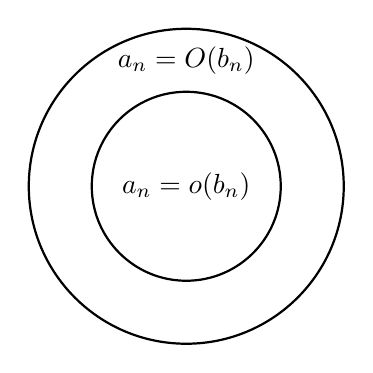
\begin{tikzpicture}
\draw[thick] (0,0) circle (2);
\draw[thick] (0,0) circle (1.2);
\node at (0,0) {$a_n = o(b_n)$};
\node at (0,1.6) {$a_n = O(b_n)$};
\end{tikzpicture}
\end{center}
\end{custom}

\begin{custom}{无穷小与无穷大的关系}
若 \(\{a_n\}\) 是非零无穷小量，则 \(\left\{\dfrac{1}{a_n}\right\}\) 是无穷大量；反之亦然。
\end{custom}

\begin{example}[常见无穷小量的比较]
当 \(n \to \infty\) 时：
\begin{itemize}
\item \(\dfrac{1}{n^p}\)（\(p>0\)）：\(p\) 越大，趋近 0 越快。
\item \(q^n\)（\(0 < q < 1\)）：指数衰减，比任何多项式都快。
\item \(\dfrac{1}{\ln n}\)：衰减极慢。
\item \(\dfrac{1}{n!}\)：衰减极快。
\end{itemize}

\textbf{增长率比较：} 当 \(n \to \infty\) 时，
\[
\ln n \ \ll\ n^p \ \ll\ a^n \ \ll\ n! \ \ll\ n^n \qquad (p>0,\ a>1).
\]
即：对数函数 < 幂函数 < 指数函数 < 阶乘 < \(n^n\)。
\end{example}

\begin{extra}
\subsection*{柯西收敛准则（选读）}
\begin{definition}[柯西列]
若对任意 \(\varepsilon > 0\)，存在 \(N\)，当 \(m,n > N\) 时 \(|a_m - a_n| < \varepsilon\)，则称 \(\{a_n\}\) 为柯西列。
\end{definition}
在实数集中，柯西列必收敛（这等价于实数的完备性）。柯西准则的好处是：判断收敛性时不需要知道极限值。
\end{extra}

\subsection*{练习题：数列极限的严格定义}

\begin{exercise}
用 \(\varepsilon\)-\(N\) 语言来说明这些数列的极限。
\begin{enumerate}
\item \(\lim\limits_{n\to\infty} \dfrac{3}{n} = 0\)
\item \(\lim\limits_{n\to\infty} \dfrac{1}{\sqrt{n}} = 0\)
\item \(\lim\limits_{n\to\infty} \dfrac{5n-2}{n+1} = 5\)
\end{enumerate}
\end{exercise}

\begin{exercise}
\begin{enumerate}
\item 如果数列 \(\{a_n\}\) 收敛，它的极限是否唯一？请简要说明理由。
\item 若 \(\lim\limits_{n\to\infty} a_n = 3\)，证明：存在正整数 \(N\)，使得当 \(n > N\) 时，\(a_n > 2\)。
\item 证明：若数列 \(\{a_n\}\) 收敛，则它必有界。（提示：取 \(\varepsilon = 1\)）
\end{enumerate}
\end{exercise}

\begin{exercise}
\begin{enumerate}
\item 判断下列数列是否为无穷小量：
   \[
   a_n = \dfrac{(-1)^n}{n},\quad b_n = \dfrac{n}{n+1},\quad c_n = 0.99^n,\quad d_n = \ln\left(1+\dfrac{1}{n}\right)
   \]
\item 判断下列数列是否为无穷大量：
   \[
   a_n = n^2,\quad b_n = (-1)^n n,\quad c_n = \ln n,\quad d_n = \dfrac{n^2}{n+1}
   \]
\item 若 \(\{a_n\}\) 是无穷小量且 \(a_n \neq 0\)，证明 \(\left\{\dfrac{1}{a_n}\right\}\) 是无穷大量。
\end{enumerate}
\end{exercise}

\begin{exercise}
用 \(\varepsilon\)-\(N\) 定义证明下列极限：
\begin{enumerate}
\item \(\lim\limits_{n\to\infty} \dfrac{\sin n}{n^2 + 1} = 0\)（提示：\(|\sin n| \leq 1\)）
\item \(\lim\limits_{n\to\infty} \dfrac{3n + \cos n}{2n - 1} = \dfrac{3}{2}\)（提示：先分拆，再放缩）
\end{enumerate}
\end{exercise}

\begin{exercise}
用 \(\varepsilon\)-\(N\) 定义证明：
\[
\lim_{n\to\infty} \left(\sqrt{n^2 + n} - n\right) = \dfrac{1}{2}.
\]
（提示：分子有理化后处理）
\end{exercise}

\begin{exercise}
设常数 \(c > 0\)，证明：
\[
\lim_{n\to\infty} \dfrac{n^c}{a^n} = 0 \quad (a > 1).
\]
（提示：当 \(n\) 足够大时，\(a^n\) 增长快于任何幂函数；可用二项式定理或取对数）
\end{exercise}

\begin{exercise}
证明下列数列发散（极限不存在）：
\begin{enumerate}
\item \(a_n = (-1)^n\)
\item \(a_n = \sin\left(\dfrac{n\pi}{2}\right)\)
\item \(a_n = n + (-1)^n n\)（提示：考虑偶子列和奇子列）
\end{enumerate}
\end{exercise}

\begin{exercise}
用 \(\varepsilon\)-\(N\) 定义证明：
\[
\lim_{n\to\infty} \dfrac{n^2 - 2n + 3}{2n^2 + 5} = \dfrac{1}{2}.
\]
要求明确给出 \(N\) 关于 \(\varepsilon\) 的表达式（可分段处理）。
\end{exercise}

\begin{exercise}
用 \(\varepsilon\)-\(N\) 定义证明：
\begin{enumerate}
\item \(\lim\limits_{n\to\infty} \dfrac{\ln n}{n} = 0\)（提示：对任意 \(\varepsilon > 0\)，取 \(N = \lceil e^{1/\varepsilon} \rceil\) 是否可行？需要调整）
\item \(\lim\limits_{n\to\infty} \sqrt[n]{n} = 1\)（提示：设 \(\sqrt[n]{n} = 1 + h_n\)，利用二项式定理证明 \(h_n \to 0\)）
\end{enumerate}
\end{exercise}

\begin{exercise}
设 \(a_n = \dfrac{1}{n^2 + 1} + \dfrac{1}{n^2 + 2} + \cdots + \dfrac{1}{n^2 + n}\)。
\begin{enumerate}
\item 证明：\(\dfrac{n}{n^2 + n} \leq a_n \leq \dfrac{n}{n^2 + 1}\)。
\item 利用夹逼准则求 \(\lim\limits_{n\to\infty} a_n\)。
\item 用 \(\varepsilon\)-\(N\) 定义直接证明该极限。（选做）
\end{enumerate}
\end{exercise}

\begin{exercise}[*（柯西收敛准则）]
设数列 \(\{a_n\}\) 满足：对任意 \(n\)，有 \(|a_{n+1} - a_n| \leq \dfrac{1}{2^n}\)。
\begin{enumerate}
\item 证明：对任意 \(m > n\)，有 \(|a_m - a_n| \leq \dfrac{1}{2^{n-1}}\)。（提示：用三角不等式和等比数列求和）
\item 证明：\(\{a_n\}\) 是柯西列，从而收敛。
\item 若已知 \(a_1 = 1\)，能否求出 \(\lim\limits_{n\to\infty} a_n\)？为什么？
\end{enumerate}
\end{exercise}


\subsection*{参考答案提要}

\begin{enumerate}
\item[(1)] 
   (a) \(N = \lceil 3/\varepsilon \rceil\)；(b) \(N = \lceil 1/\varepsilon^2 \rceil\)；(c) \(\left|\dfrac{5n-2}{n+1} - 5\right| = \dfrac{7}{n+1}\)，取 \(N = \lceil 7/\varepsilon \rceil\)。

\item[(2)] 
   (a) 唯一，反证法用 \(\varepsilon = |L_1 - L_2|/2\) 导出矛盾；(b) 取 \(\varepsilon = 1\)，存在 \(N\) 使 \(n > N\) 时 \(|a_n-3|<1\)，故 \(a_n > 2\)；(c) 取 \(\varepsilon=1\)，有界性证明略。

\item[(3)] 
   (a) 无穷小量：\(a_n, c_n, d_n\)（\(b_n \to 1\) 不是）；(b) 无穷大量：\(a_n, c_n, d_n\)（\(b_n\) 无界但不趋于无穷）；(c) 由定义直接验证。

\item[(4)] 
   (a) \(\left|\dfrac{\sin n}{n^2+1}\right| \leq \dfrac{1}{n^2}\)，取 \(N = \lceil 1/\sqrt{\varepsilon} \rceil\)；(b) 先化简为 \(\dfrac{3}{2} + \dfrac{3\cos n + 3/2}{2(2n-1)}\) 再放缩。

\item[(5)] 
   分子有理化：\(\sqrt{n^2+n} - n = \dfrac{n}{\sqrt{n^2+n}+n} = \dfrac{1}{\sqrt{1+1/n}+1}\)，然后放缩证明。

\item[(6)] 
   令 \(a_n = n^c / a^n\)，当 \(n > 2c\) 时可用二项式定理 \((1+(a-1))^n \geq \binom{n}{2}(a-1)^2\) 放缩。

\item[(7)] 
   (a) 子列极限不同；(b) 子列 \(0,1,0,-1,\dots\) 不收敛；(c) \(a_n = n(1+(-1)^n)\)，偶数项 \(\to +\infty\)，奇数项为 0。

\item[(8)] 
   \(\left|\dfrac{n^2-2n+3}{2n^2+5} - \dfrac{1}{2}\right| = \dfrac{4n+1}{2(2n^2+5)} < \dfrac{4n+1}{4n^2} < \dfrac{5}{4n}\)（当 \(n \geq 1\)），取 \(N = \lceil 5/(4\varepsilon) \rceil\)。

\item[(9)] 
   (a) 取 \(N = \lceil e^{2/\varepsilon} \rceil\) 或通过 \(n > e^{1/\varepsilon}\) 放缩；(b) 由 \(\sqrt[n]{n} = 1+h_n\)，二项展开得 \(n = (1+h_n)^n \geq \binom{n}{2}h_n^2\)，故 \(h_n^2 \leq \dfrac{2}{n-1} \to 0\)。

\item[(10)] 
   (a) 左边放缩：每项 \(\geq \dfrac{1}{n^2+n}\)，共 \(n\) 项；右边放缩：每项 \(\leq \dfrac{1}{n^2+1}\)；(b) 夹逼得极限为 0；(c) 直接证明：\(0 \leq a_n \leq \dfrac{1}{n}\)，取 \(N = \lceil 1/\varepsilon \rceil\)。

\item[(11)] 
   (a) \(|a_m - a_n| \leq \sum_{k=n}^{m-1} |a_{k+1}-a_k| \leq \sum_{k=n}^{\infty} \dfrac{1}{2^k} = \dfrac{1}{2^{n-1}}\)；(b) 由 (a) 知 \(\{a_n\}\) 是柯西列，故收敛；(c) 不能，因为只知道差值大小，不知道具体值。
\end{enumerate}
\end{custom}

\clearpage
\section{极限的性质与重要极限}

\subsection{收敛数列的基本性质}

\begin{theorem}[极限的性质]
设 \(\{a_n\}, \{b_n\}\) 为收敛数列。
\begin{enumerate}
\item \textbf{唯一性：} 收敛数列极限唯一。
\item \textbf{保号性：} 若当 \(n\) 充分大时 \(a_n \geq 0\)，且 \(\lim a_n = L\)，则 \(L \geq 0\)。
\item \textbf{有界性：} 收敛数列必有界。
\item \textbf{夹逼准则（三明治定理）：} 若 \(b_n \leq a_n \leq c_n\)（当 \(n\) 充分大）且 \(\lim b_n = \lim c_n = L\)，则 \(\lim a_n = L\)。
\item \textbf{四则运算：}
   \begin{align*}
   \lim (c_1 a_n + c_2 b_n) &= c_1 \lim a_n + c_2 \lim b_n,\\
   \lim (a_n b_n) &= (\lim a_n)(\lim b_n),\\
   \lim \dfrac{a_n}{b_n} &= \dfrac{\lim a_n}{\lim b_n} \quad (\lim b_n \neq 0).
   \end{align*}
\end{enumerate}
\end{theorem}

\begin{custom}{唯一性的证明}
假设 \(a_n \to L_1\) 且 \(a_n \to L_2\)。对任意 \(\varepsilon > 0\)，存在 \(N_1, N_2\) 使当 \(n > \max(N_1, N_2)\) 时，
\[
|a_n - L_1| < \varepsilon,\quad |a_n - L_2| < \varepsilon.
\]
于是
\[
|L_1 - L_2| \leq |L_1 - a_n| + |a_n - L_2| < 2\varepsilon.
\]
由于 \(\varepsilon\) 可以任意小，而 \(|L_1 - L_2|\) 是常数，故 \(L_1 = L_2\)。\(\square\)
\end{custom}

\begin{custom}{保号性的证明}
假设 \(\lim a_n = L < 0\)。取 \(\varepsilon = -L/2 > 0\)，则存在 \(N\)，当 \(n > N\) 时 \(|a_n - L| < -L/2\)，从而 \(a_n < L/2 < 0\)，与 \(a_n \geq 0\) 矛盾。故 \(L \geq 0\)。\(\square\)
\end{custom}

\begin{custom}{有界性的证明}
设 \(\lim a_n = L\)。取 \(\varepsilon = 1\)，存在 \(N\)，当 \(n > N\) 时 \(|a_n - L| < 1\)，故 \(|a_n| < |L| + 1\)。取
\[
M = \max\{|a_1|, |a_2|, \dots, |a_N|, |L|+1\},
\]
则对所有 \(n\) 有 \(|a_n| \leq M\)。\(\square\)
\end{custom}

\begin{custom}{夹逼准则的证明}
由 \(\lim b_n = L\)，对 \(\varepsilon > 0\)，存在 \(N_1\) 使 \(n > N_1\) 时 \(L - \varepsilon < b_n < L + \varepsilon\)。
由 \(\lim c_n = L\)，存在 \(N_2\) 使 \(n > N_2\) 时 \(L - \varepsilon < c_n < L + \varepsilon\)。
取 \(N = \max(N_1, N_2)\)，则当 \(n > N\) 时，
\[
L - \varepsilon < b_n \leq a_n \leq c_n < L + \varepsilon,
\]
故 \(|a_n - L| < \varepsilon\)，即 \(\lim a_n = L\)。\(\square\)
\end{custom}

\begin{custom}{四则运算的证明思路}
以乘法为例：设 \(a_n \to A\)，\(b_n \to B\)。则
\[
a_n b_n - AB = (a_n - A)b_n + A(b_n - B).
\]
由于 \(b_n\) 有界，\(a_n - A \to 0\)，故第一项趋于 0；第二项也趋于 0。因此 \(a_n b_n \to AB\)。
\end{custom}

\subsection{Landau 符号的四则运算性质}

在极限计算和渐近分析中，小 \(o\) 和大 \(O\) 记号具有简洁的运算规则，掌握这些规则可以极大地简化极限计算。

\begin{theorem}[小 \(o\) 与大 \(O\) 的运算性质]
设 \(f(x), g(x), h(x)\) 是定义在某个邻域内的函数（或数列），且 \(x \to x_0\)（或 \(n \to \infty\)）。则以下运算规则成立：

\begin{enumerate}
\item \textbf{常数倍：}
   \[
   c \cdot o(g) = o(g),\quad c \cdot O(g) = O(g) \quad (c \text{ 为非零常数})
   \]

\item \textbf{加减法：}
   \[
   o(g) + o(g) = o(g),\quad O(g) + O(g) = O(g)
   \]
   \[
   o(g) - o(g) = o(g),\quad O(g) - O(g) = O(g)
   \]
   \[
   o(g) + O(g) = O(g) \quad (\text{但通常不能写成 } o(g))
   \]

\item \textbf{乘法：}
   \[
   o(g) \cdot o(h) = o(gh),\quad O(g) \cdot O(h) = O(gh)
   \]
   \[
   o(g) \cdot O(h) = o(gh),\quad O(g) \cdot o(h) = o(gh)
   \]

\item \textbf{传递性：}
   \begin{itemize}
   \item 若 \(f = o(g)\) 且 \(g = o(h)\)，则 \(f = o(h)\)
   \item 若 \(f = O(g)\) 且 \(g = O(h)\)，则 \(f = O(h)\)
   \item 若 \(f = o(g)\) 且 \(g = O(h)\)，则 \(f = o(h)\)
   \end{itemize}

\item \textbf{与极限的关系：}
   \begin{itemize}
   \item \(f(x) \to 0\) 当且仅当 \(f(x) = o(1)\)
   \item \(f(x)\) 有界当且仅当 \(f(x) = O(1)\)
   \end{itemize}

\item \textbf{主要项法则：} 若 \(f = o(g)\)，则 \(f + g \sim g\)（即 \(f+g\) 与 \(g\) 是等价无穷小）
\end{enumerate}
\end{theorem}

\begin{custom}{规则背后的直观理解}

这些规则其实很符合直觉：

\begin{itemize}
\item \textbf{加法规则：} 两个“小东西”加起来还是“小东西”；两个“有界的东西”加起来还是有界的。
\item \textbf{乘法规则：} “小东西”乘以“小东西”更小（高阶乘高阶得更高阶）；“小东西”乘以“有界的东西”还是小东西。
\item \textbf{传递性：} 如果 \(f\) 比 \(g\) 小得多，\(g\) 比 \(h\) 小得多，那么 \(f\) 比 \(h\) 小得多。
\end{itemize}

\textbf{一个容易混淆的点：} \(o(g) + O(g) = O(g)\)，但不能写成 \(o(g)\)。因为 \(O(g)\) 可能包含一个与 \(g\) 同阶的项（比如 \(g\) 本身），而 \(o(g)\) 要求比值趋于 0，所以 \(g\) 本身不是 \(o(g)\)。
\end{custom}


\begin{example}[利用 o 和 O 比较数列增长]
比较下列数列的增长速度：
\[
a_n = n^2 + n \ln n,\quad b_n = n^2.
\]

\begin{custom}{解}
\[
a_n = n^2 + n \ln n = n^2 \left(1 + \dfrac{\ln n}{n}\right).
\]
由于 \(\dfrac{\ln n}{n} = o(1)\)，所以
\[
a_n = n^2 (1 + o(1)) = n^2 + o(n^2).
\]
因此 \(a_n \sim n^2\)，即 \(a_n\) 与 \(b_n\) 是等价无穷大（当 \(n \to \infty\)）。
\end{custom}
\end{example}

\begin{custom}{常见错误警示}

\begin{tabular}{|c|c|c|}
\hline
\textbf{错误写法} & \textbf{问题} & \textbf{正确理解} \\
\hline
\(o(g) - o(g) = 0\) & 两个不同的 \(o(g)\) 相减不一定为 0 & \(o(g) - o(g) = o(g)\) \\
\hline
\(\dfrac{o(g)}{g} = 0\) & 写法不规范 & 应写为 \(\dfrac{o(g)}{g} \to 0\) \\
\hline
\(o(1) \cdot \infty = ?\) & 未定义 & \(o(1)\) 乘以无穷大可能为任何情况 \\
\hline
\(\sin x = x + O(x^3)\) 与 \(\sin x = x + o(x^2)\) 混淆 & 精度不同 & \(O(x^3)\) 比 \(o(x^2)\) 提供更多信息 \\
\hline
\end{tabular}

\textbf{核心原则：} 小 \(o\) 描述的是“比……高阶”，大 \(O\) 描述的是“不超过……的常数倍”。在运算中，小 \(o\) 会“吸收”比自己低阶或同阶的项，而大 \(O\) 只保证有界性。
\end{custom}

\subsection{极限存在性定理}

有时候我们不知道极限值，但仍能判断极限是否存在。

\begin{theorem}[单调有界准则]
单调递增且有上界的数列必收敛；单调递减且有下界的数列必收敛。
\end{theorem}

\begin{custom}{直观理解}
想象一个人在数轴上向右走（单调递增），但前面有一堵墙（上界）。他不能无限向右，只能越来越靠近某个点。这个点就是极限。
\end{custom}

\begin{example}[重要例子]
证明数列 \(a_1 = \sqrt{2}\)，\(a_{n+1} = \sqrt{2 + a_n}\) 收敛并求极限。
\end{example}
\begin{custom}{解}
\textbf{有界性：} \(a_1 = \sqrt{2} < 2\)，假设 \(a_k < 2\)，则 \(a_{n+1} = \sqrt{2 + a_n} < \sqrt{4} = 2\)，故 \(a_n < 2\) 对所有 \(n\) 成立。
\textbf{单调性：} \(a_2 = \sqrt{2+\sqrt{2}} > \sqrt{2} = a_1\)，假设 \(a_k > a_{k-1}\)，则 \(a_{k+1} = \sqrt{2 + a_k} > \sqrt{2 + a_{k-1}} = a_k\)，故 \(\{a_n\}\) 严格递增。
由单调有界准则，极限存在。设 \(\lim a_n = L\)，在递推式两边取极限：
\[
L = \sqrt{2 + L} \quad\Longrightarrow\quad L^2 = L + 2 \quad\Longrightarrow\quad L = 2\ (\text{舍去 } -1).
\]
\end{custom}

\begin{theorem}[Bolzano-Weierstrass定理]
\textbf{（有界数列必有收敛子列）}
任何有界数列 \(\{a_n\}\) 必定存在一个收敛的子列 \(\{a_{n_k}\}\)。
\end{theorem}

\begin{custom}{直观理解}

这个定理说的是：如果你有一列数，它们都挤在某个有限的区间里（比如都在 \([-M, M]\) 之间），那么无论它们看起来多么杂乱无章，你总能从中挑出一个“收敛”的子序列。

\textbf{一个生活中的比喻：}

想象一个无限大的体育馆里有无穷多个人，每个人手里拿着一个数字，所有数字都在 0 到 1 之间。你想找出一群人，他们手里的数字越来越接近某个固定值。

Bolzano-Weierstrass 定理保证：你一定能找到这样一群人！无论这些人怎么站队，你总能挑出一个子序列，它最终会稳定在某个数附近。

\textbf{一个更直观的几何解释：}

把数列 \(\{a_n\}\) 想象成数轴上的无限个点，所有点都被关在区间 \([-M, M]\) 这个“笼子”里。

\begin{center}
\begin{tikzpicture}[scale=0.8]
\draw[thick, -{Stealth}] (-5,0) -- (5,0) node[right] {数轴};
\draw[thick] (-4,0.1) -- (-4,-0.1) node[below] {\(-M\)};
\draw[thick] (4,0.1) -- (4,-0.1) node[below] {\(M\)};
\draw[thick, red] (-4,0.2) -- (4,0.2) node[above] {笼子（有界区间）};

\foreach \x in {-3.2, -1.5, -0.8, 0.3, 1.2, 2.5, 3.7, -2.1, 0.9, 2.8, -0.2, 1.9, -2.9, 3.1} {
    \filldraw[blue] (\x,0) circle (2pt);
}
\end{tikzpicture}
\end{center}

\textbf{核心思想——二分法：}

你可以用“不断对半分割区间”的方法来构造这个收敛子列：

\begin{enumerate}
\item 一开始，所有点都在区间 \([a, b] = [-M, M]\) 里。
\item 把这个区间分成两半：左边 \([-M, 0]\) 和右边 \([0, M]\)。由于有无穷多个点，至少有一半包含无穷多个点。选择那一半作为新区间 \([a_1, b_1]\)。
\item 再把新区间对半分，同样，至少有一半包含无穷多个点。选择那一半作为 \([a_2, b_2]\)。
\item 如此无限继续下去，我们得到一列不断缩小的区间：
\[
[a, b] \supset [a_1, b_1] \supset [a_2, b_2] \supset \cdots
\]
\item 每次区间的长度减半：\(b_n - a_n = \dfrac{2M}{2^n} \to 0\)。
\item 从每个区间里选出一个数列中的点 \(a_{n_k}\)，这些点就构成了一个收敛的子列。这些点被“挤压”在越来越小的区间里，最终会收敛到区间的公共极限点 \(c\)。
\end{enumerate}

\textbf{一个具体的例子：}

考虑数列 \(a_n = \sin n\)。虽然 \(\sin n\) 在 \([-1, 1]\) 之间振荡，看起来毫无规律，但 Bolzano-Weierstrass 定理告诉我们：一定存在一个子列收敛。事实上，可以证明 \(\sin n\) 的子列可以收敛到 \([-1, 1]\) 中的任意值，但这个定理只保证“存在”，不告诉我们具体是哪个。

\end{custom}

\begin{custom}{单调有界准则 vs Bolzano-Weierstrass 定理}

这两个定理是实数完备性的不同表现形式，它们实际上是等价的（在实数系中可以互相推导）。

\begin{tabular}{|c|c|c|}
\hline
 & \textbf{单调有界准则} & \textbf{Bolzano-Weierstrass 定理} \\
\hline
\textbf{条件} & 数列单调 + 有界 & 数列有界（不要求单调） \\
\hline
\textbf{结论} & 数列本身收敛 & 存在收敛子列 \\
\hline
\textbf{适用场景} & 单调数列 & 任意有界数列 \\
\hline
\textbf{直观比喻} & 向右走，前面有墙 & 笼子里的无限多只鸟 \\
\hline
\end{tabular}

\textbf{关系：}
\begin{itemize}
\item 单调有界准则更强：它直接得出数列本身收敛。
\item Bolzano-Weierstrass 更广：它适用于任何有界数列，但只给出子列收敛。
\item 如果数列既有界又单调，两个定理都适用，但单调有界准则给出的结论更强。
\end{itemize}

\end{custom}


\begin{example}[重要例子]
证明数列 \(a_1 = \sqrt{2}\)，\(a_{n+1} = \sqrt{2 + a_n}\) 收敛并求极限。
\end{example}
\begin{custom}{解}
\textbf{有界性：} \(a_1 = \sqrt{2} < 2\)，假设 \(a_k < 2\)，则 \(a_{k+1} = \sqrt{2 + a_k} < \sqrt{4} = 2\)，故 \(a_n < 2\) 对所有 \(n\) 成立。
\textbf{单调性：} \(a_2 = \sqrt{2+\sqrt{2}} > \sqrt{2} = a_1\)，假设 \(a_k > a_{k-1}\)，则 \(a_{k+1} = \sqrt{2 + a_k} > \sqrt{2 + a_{k-1}} = a_k\)，故 \(\{a_n\}\) 严格递增。
由单调有界准则，极限存在。设 \(\lim a_n = L\)，在递推式两边取极限：
\[
L = \sqrt{2 + L} \quad\Longrightarrow\quad L^2 = L + 2 \quad\Longrightarrow\quad L = 2\ (\text{舍去 } -1).
\]
\end{custom}

\subsection{两个重要极限}

\begin{theorem}[第一个重要极限]
\[
\lim_{n\to\infty} \left(1 + \dfrac{1}{n}\right)^n = e.
\]
\end{theorem}

\textbf{故事背景：} 17世纪，数学家雅各布·伯努利在研究复利问题时遇到了这个极限。假设你存 1 元钱，年利率 100\%，如果一年计一次息，本息和为 2 元；如果半年计一次，本息和为 \((1+0.5)^2 = 2.25\)；如果每月计一次，为 \((1+1/12)^{12} \approx 2.613\)；如果每天计一次，约为 \(2.71457\)。这个数的极限就是 \(e \approx 2.71828\ldots\)。

\begin{custom}{具体证明}
证明分为两步：先证 \(\{a_n\}\) 单调递增，再证它有上界。

\noindent\textbf{第一步：证明单调递增}

由二项式定理展开：
\[
a_n = \left(1+\dfrac{1}{n}\right)^n = \sum_{k=0}^{n} C_n^k \dfrac{1}{n^k} = \sum_{k=0}^{n} \dfrac{1}{k!} \cdot \dfrac{n(n-1)\cdots(n-k+1)}{n^k}.
\]
其中 \(\dfrac{n(n-1)\cdots(n-k+1)}{n^k} = 1 \cdot \left(1-\dfrac{1}{n}\right) \cdots \left(1-\dfrac{k-1}{n}\right)\)。于是
\[
a_n = \sum_{k=0}^{n} \dfrac{1}{k!} \left(1-\dfrac{1}{n}\right)\left(1-\dfrac{2}{n}\right)\cdots\left(1-\dfrac{k-1}{n}\right).
\]

同理，
\[
a_{n+1} = \sum_{k=0}^{n+1} \dfrac{1}{k!} \left(1-\dfrac{1}{n+1}\right)\left(1-\dfrac{2}{n+1}\right)\cdots\left(1-\dfrac{k-1}{n+1}\right).
\]

比较 \(a_n\) 与 \(a_{n+1}\) 中 \(k\) 相同的项（\(1 \leq k \leq n\)）：
\[
\left(1-\dfrac{1}{n}\right)\left(1-\dfrac{2}{n}\right)\cdots\left(1-\dfrac{k-1}{n}\right) < \left(1-\dfrac{1}{n+1}\right)\left(1-\dfrac{2}{n+1}\right)\cdots\left(1-\dfrac{k-1}{n+1}\right),
\]
因为每个因子 \(1-\dfrac{j}{n} < 1-\dfrac{j}{n+1}\)（\(j=1,2,\dots,k-1\)）。同时 \(a_{n+1}\) 比 \(a_n\) 多一项正的 \(\dfrac{1}{(n+1)!}\)。因此
\[
a_n < a_{n+1},
\]
故数列严格递增。

\noindent\textbf{第二步：证明有上界}

由展开式，
\[
a_n = \sum_{k=0}^{n} \dfrac{1}{k!} \left(1-\dfrac{1}{n}\right)\cdots\left(1-\dfrac{k-1}{n}\right) < \sum_{k=0}^{n} \dfrac{1}{k!}.
\]

当 \(k \geq 1\) 时，\(k! = 1 \cdot 2 \cdot 3 \cdots k \geq 1 \cdot 2 \cdot 2 \cdots 2 = 2^{k-1}\)，因此
\[
\dfrac{1}{k!} \leq \dfrac{1}{2^{k-1}} \quad (k \geq 1).
\]

于是
\[
a_n < 1 + 1 + \dfrac{1}{2} + \dfrac{1}{2^2} + \cdots + \dfrac{1}{2^{n-1}} = 1 + \dfrac{1 - (1/2)^n}{1 - 1/2} = 1 + 2\left(1 - \dfrac{1}{2^n}\right) < 3.
\]

所以 \(a_n < 3\) 对所有 \(n\) 成立，数列有上界。

\noindent\textbf{结论：} 数列 \(\{a_n\}\) 单调递增且有上界，由单调有界准则，极限存在。记这个极限为 \(e\)，即
\[
e = \lim_{n\to\infty} \left(1+\dfrac{1}{n}\right)^n.
\]
\end{custom}

\begin{theorem}[第一个重要极限的推广]
\[
\lim_{n\to\infty} \left(1 + \dfrac{a}{n}\right)^n = e^a.
\]
特别地，\(\lim_{x\to 0} (1+x)^{1/x} = e\)。
\end{theorem}

\subsection{重要极限 \(\lim_{x \to 0} \dfrac{\sin x}{x} = 1\)}

这个极限是微积分中最重要的极限之一。它告诉我们：当 \(x\) 非常接近 0 时，\(\sin x\) 和 \(x\) 几乎相等。

\begin{custom}{几何直观：从单位圆看起}

画一个半径为 1 的圆（单位圆）。在圆中取一个很小的角 \(x\)，如图：

\begin{center}
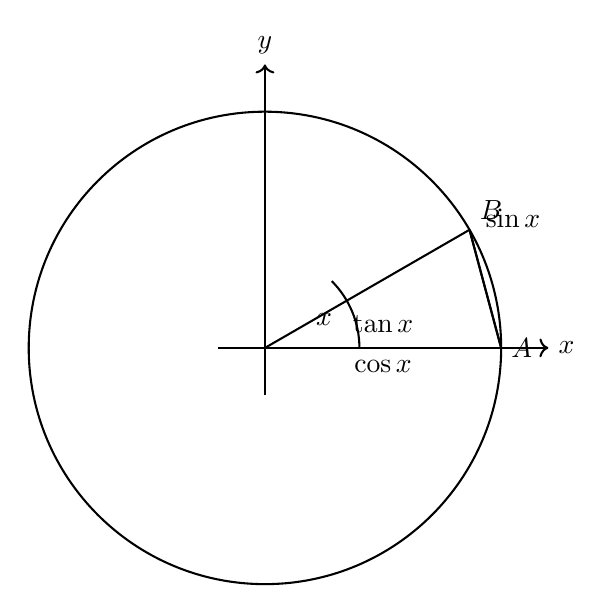
\begin{tikzpicture}[scale=3]
\draw[->] (-0.2,0) -- (1.2,0) node[right] {$x$};
\draw[->] (0,-0.2) -- (0,1.2) node[above] {$y$};
\draw (0,0) circle (1);
\draw (0,0) -- (1,0) node[right] {$A$};
\draw (0,0) -- ({cos(30)},{sin(30)}) node[above right] {$B$};
\draw (1,0) -- ({cos(30)},{sin(30)});
\draw ({cos(0.8)},0) -- ({cos(30)},{sin(30)});
\draw (0.4,0) arc (0:45:0.4);
\node at (0.25,0.12) {$x$};
\node at (0.5,0.1) {$\tan x$};
\node at (1.05,0.55) {$\sin x$};
\node at (0.5,-0.08) {$\cos x$};
\end{tikzpicture}
\end{center}

图中：
\begin{itemize}
\item 角 \(x\) 对应的圆弧长 = \(x\)（因为半径=1，弧长=半径×角度）
\item 垂线 \(BC\) 的长度 = \(\sin x\)
\item 水平线 \(AC\) 的长度 = \(\cos x\)
\item 切线 \(AD\) 的长度 = \(\tan x\)
\end{itemize}

从图中可以看出，三个面积之间有如下关系：

\[
\triangle OAB \text{ 的面积 } < \text{ 扇形 } OAB \text{ 的面积 } < \triangle OAD \text{ 的面积}.
\]

\end{custom}

\begin{custom}{面积比较}

\begin{itemize}
\item \(\triangle OAB\) 的面积 = \(\dfrac{1}{2} \times 1 \times \sin x = \dfrac{1}{2} \sin x\)
\item 扇形 \(OAB\) 的面积 = \(\dfrac{1}{2} \times 1^2 \times x = \dfrac{x}{2}\)
\item \(\triangle OAD\) 的面积 = \(\dfrac{1}{2} \times 1 \times \tan x = \dfrac{1}{2} \tan x\)
\end{itemize}

因此：

\[
\dfrac{1}{2} \sin x  <  \dfrac{x}{2} < \dfrac{1}{2} \tan x \qquad (0 < x < \dfrac{\pi}{2}).
\]

两边同时乘以 2，得到：

\[
\sin x  < x < \tan x.
\]

\end{custom}

\begin{custom}{推导 \(\dfrac{\sin x}{x}\) 的夹逼不等式}

由 \(x < \tan x = \dfrac{\sin x}{\cos x}\)，两边同时除以 \(\sin x > 0\)，得：

\[
\dfrac{x}{\sin x} < \dfrac{1}{\cos x} \quad \Longrightarrow \quad \cos x < \dfrac{\sin x}{x}.
\]

又由 \(\sin x < x\)，两边除以 \(x > 0\)，得：

\[
\dfrac{\sin x}{x} < 1.
\]

合起来：

\[
\cos x < \dfrac{\sin x}{x} < 1 \qquad (0 < x < \dfrac{\pi}{2}).
\]

\end{custom}

\begin{custom}{用夹逼准则取极限}

我们知道 \(\lim_{x \to 0} \cos x = 1\)。因此，当 \(x \to 0^+\) 时：

\[
\cos x \;\longrightarrow\; 1,\quad \dfrac{\sin x}{x} \;\longrightarrow\; 1.
\]

当 \(x\) 为负时（即 \(x \to 0^-\)），由于 \(\dfrac{\sin x}{x}\) 是偶函数（\(\sin(-x)/(-x) = \sin x / x\)），左右极限相等。因此：

\[
\lim_{x \to 0} \dfrac{\sin x}{x} = 1.
\]

\end{custom}

\begin{custom}{直观理解}

这个极限告诉我们：当角度 \(x\) 非常小时，\(\sin x\) 和 \(x\) 几乎相等。例如：

\[
x = 0.1 \text{ 弧度} \approx 5.73^\circ,\quad \sin(0.1) \approx 0.099833,\quad \dfrac{\sin 0.1}{0.1} \approx 0.99833.
\]

\[
x = 0.01 \text{ 弧度},\quad \dfrac{\sin 0.01}{0.01} \approx 0.999983.
\]

误差非常小，且随 \(x\) 越小越接近 1。

\end{custom}

\subsection{等价无穷小}

在计算极限时，我们经常遇到两个无穷小量相乘或相除的情况。如果能用一个简单的无穷小量代替复杂的无穷小量，计算会大大简化。这就是等价无穷小的思想。

\begin{definition}[等价无穷小]
设当 \(x \to x_0\)（或 \(x \to \infty\)）时，\(\alpha(x) \to 0\)，\(\beta(x) \to 0\)，且
\[
\lim \dfrac{\alpha(x)}{\beta(x)} = 1,
\]
则称 \(\alpha(x)\) 与 \(\beta(x)\) 是等价无穷小，记作 \(\alpha(x) \sim \beta(x)\)。
\end{definition}

\begin{custom}{直观理解}
等价无穷小意味着：当两个量都趋近于 0 时，它们的比值趋近于 1，即它们“以相同的速度”趋近于 0。

打个比方：两辆赛车同时冲向终点，如果它们速度相同，那么它们之间的距离会越来越小，最终几乎同时到达。等价无穷小就是这种“同步趋近”的数学描述。
\end{custom}

\subsection{常用等价无穷小（\(x \to 0\) 时）}

以下等价关系是微积分中最常用的，务必熟记：

\[
\boxed{
\begin{aligned}
\sin x &\sim x & \tan x &\sim x \\
\arcsin x &\sim x & \arctan x &\sim x \\
e^x - 1 &\sim x & \ln(1+x) &\sim x \\
1 - \cos x &\sim \dfrac{x^2}{2} & (1+x)^a - 1 &\sim ax \quad (a \neq 0)
\end{aligned}
}
\]

\begin{custom}{几个等价关系的推导}

\begin{itemize}
\item \textbf{\(\sin x \sim x\)：} 这就是我们之前证明的 \(\lim_{x \to 0} \dfrac{\sin x}{x} = 1\)。

\item \textbf{\(\tan x \sim x\)：} 
\[
\lim_{x \to 0} \dfrac{\tan x}{x} = \lim_{x \to 0} \dfrac{\sin x}{x} \cdot \dfrac{1}{\cos x} = 1 \cdot 1 = 1.
\]

\item \textbf{\(e^x - 1 \sim x\)：} 令 \(t = e^x - 1\)，则 \(x = \ln(1+t)\)，当 \(x \to 0\) 时 \(t \to 0\)，
\[
\lim_{x \to 0} \dfrac{e^x - 1}{x} = \lim_{t \to 0} \dfrac{t}{\ln(1+t)} = 1.
\]

\item \textbf{\(\ln(1+x) \sim x\)：} 
\[
\lim_{x \to 0} \dfrac{\ln(1+x)}{x} = \lim_{x \to 0} \ln(1+x)^{1/x} = \ln e = 1.
\]

\item \textbf{\(1 - \cos x \sim \dfrac{x^2}{2}\)：} 
\[
\lim_{x \to 0} \dfrac{1 - \cos x}{x^2/2} = \lim_{x \to 0} \dfrac{2 \sin^2(x/2)}{x^2/2} = \lim_{x \to 0} \dfrac{4 \sin^2(x/2)}{x^2} = \lim_{x \to 0} \left(\dfrac{\sin(x/2)}{x/2}\right)^2 = 1.
\]

\item \textbf{\((1+x)^a - 1 \sim ax\)：} 
\[
\lim_{x \to 0} \dfrac{(1+x)^a - 1}{ax} = \dfrac{1}{a} \cdot \lim_{x \to 0} \dfrac{e^{a\ln(1+x)} - 1}{x} = \dfrac{1}{a} \cdot \lim_{x \to 0} \dfrac{a\ln(1+x)}{x} = 1.
\]
\end{itemize}
\end{custom}

\subsection{等价无穷小的应用：简化极限计算}

\begin{custom}{核心原则}
在乘除结构中，可以用等价无穷小替换来简化计算：
\[
\lim \dfrac{f(x)}{g(x)} = \lim \dfrac{\tilde{f}(x)}{\tilde{g}(x)},
\]
其中 \(\tilde{f} \sim f\)，\(\tilde{g} \sim g\)。

\textbf{但注意：} 在加减结构中，不能随意替换！因为主要项可能相互抵消，替换后可能丢失关键信息。
\end{custom}

\begin{example}[乘除结构中的替换]
求 \(\lim\limits_{x \to 0} \dfrac{\sin 2x \cdot \ln(1+3x)}{x^2}\)。
\end{example}
\begin{custom}{解}
当 \(x \to 0\) 时，\(\sin 2x \sim 2x\)，\(\ln(1+3x) \sim 3x\)，所以
\[
\dfrac{\sin 2x \cdot \ln(1+3x)}{x^2} \sim \dfrac{(2x) \cdot (3x)}{x^2} = 6 \quad \Rightarrow \quad \text{极限为 } 6.
\]
更严谨地：
\[
\lim_{x \to 0} \dfrac{\sin 2x \cdot \ln(1+3x)}{x^2} = \lim_{x \to 0} \dfrac{\sin 2x}{2x} \cdot \dfrac{\ln(1+3x)}{3x} \cdot 6 = 1 \cdot 1 \cdot 6 = 6.
\]
\end{custom}

\begin{example}[乘除结构中的复杂替换]
求 \(\lim\limits_{x \to 0} \dfrac{e^{x^2} - \cos x}{x^2}\)。
\end{example}
\begin{custom}{解}
这里分子是两项相减，不能直接分别替换。但可以将每一项展开：
\[
e^{x^2} = 1 + x^2 + o(x^2),\quad \cos x = 1 - \dfrac{x^2}{2} + o(x^2),
\]
所以
\[
e^{x^2} - \cos x = \left(1 + x^2 + o(x^2)\right) - \left(1 - \dfrac{x^2}{2} + o(x^2)\right) = \dfrac{3}{2}x^2 + o(x^2),
\]
因此
\[
\lim_{x \to 0} \dfrac{e^{x^2} - \cos x}{x^2} = \dfrac{3}{2}.
\]

\textbf{注意：} 这里不能直接用 \(e^{x^2} \sim 1\) 和 \(\cos x \sim 1\)，因为 \(1-1=0\) 会丢失主要信息。
\end{custom}

\begin{example}[加减结构中的错误示例]
求 \(\lim\limits_{x \to 0} \dfrac{\tan x - \sin x}{x^3}\)。

\textbf{错误解法：} \(\tan x \sim x\)，\(\sin x \sim x\)，则 \(\tan x - \sin x \sim x - x = 0\)，极限为 0。\textcolor{red}{（错误！）}

\textbf{正确解法：} 展开到三阶：
\[
\tan x = x + \dfrac{x^3}{3} + o(x^3),\quad \sin x = x - \dfrac{x^3}{6} + o(x^3),
\]
\[
\tan x - \sin x = \dfrac{x^3}{2} + o(x^3),
\]
所以极限为 \(\dfrac{1}{2}\)。

或者提取公因式：
\[
\dfrac{\tan x - \sin x}{x^3} = \dfrac{\sin x(1 - \cos x)}{x^3 \cos x} \sim \dfrac{x \cdot (x^2/2)}{x^3 \cdot 1} = \dfrac{1}{2}.
\]
\end{custom}

\begin{custom}{等价无穷小替换的口诀}
\begin{center}
\fbox{\parbox{0.85\textwidth}{
\textbf{乘除随便换，加减要谨慎。}\\
\textbf{若问为什么，展开看高阶。}}
}
\end{center}

\textbf{具体规则：}
\begin{itemize}
\item 在乘除结构中：可以用等价无穷小替换因子。
\item 在加减结构中：
  \begin{itemize}
    \item 如果两个无穷小不是同阶，可以替换（高阶可忽略）；
    \item 如果两个无穷小是同阶，替换后可能抵消主要项，必须展开到足够高阶。
  \end{itemize}
\end{itemize}
\end{custom}

\subsection{等价无穷小与无穷小量阶的比较}

为了更精确地描述无穷小量趋近于 0 的“速度”，我们引入阶的概念。

\begin{definition}[无穷小的阶]
设 \(\alpha(x) \to 0\)，\(\beta(x) \to 0\)，且 \(\beta(x) \neq 0\)。
\begin{itemize}
\item 若 \(\lim \dfrac{\alpha}{\beta} = 0\)，称 \(\alpha\) 是比 \(\beta\) 高阶的无穷小，记作 \(\alpha = o(\beta)\)。
\item 若 \(\lim \dfrac{\alpha}{\beta} = C \neq 0\)，称 \(\alpha\) 与 \(\beta\) 是同阶无穷小。
\item 特别地，若 \(C = 1\)，称 \(\alpha\) 与 \(\beta\) 是等价无穷小，记作 \(\alpha \sim \beta\)。
\end{itemize}
\end{definition}

\begin{custom}{阶的比较：举例}
当 \(x \to 0\) 时：
\begin{itemize}
\item \(x^2\) 是比 \(x\) 高阶的无穷小：\(\dfrac{x^2}{x} = x \to 0\)，记作 \(x^2 = o(x)\)。
\item \(x^2\) 与 \(2x^2\) 是同阶无穷小：\(\dfrac{x^2}{2x^2} = \dfrac{1}{2}\)。
\item \(x\) 与 \(\sin x\) 是等价无穷小：\(\dfrac{x}{\sin x} \to 1\)。
\end{itemize}

\textbf{阶的比较示意图：}
\[
\underbrace{x^3}_{o(x^2)} \quad \ll \quad \underbrace{x^2}_{o(x)} \quad \ll \quad \underbrace{x}_{\text{一阶}} \quad \ll \quad \underbrace{\sqrt{x}}_{\text{低阶}}
\]
\end{custom}


\begin{extra}
\subsection*{等价无穷小的推广（选读）}

\begin{custom}{推广一：复合函数的等价替换}
若当 \(u \to 0\) 时 \(f(u) \sim g(u)\)，且 \(u(x) \to 0\)，则当 \(x \to x_0\) 时 \(f(u(x)) \sim g(u(x))\)。

例如：\(\sin(x^2) \sim x^2\)（因为 \(x^2 \to 0\)），\(\ln(1+\sin x) \sim \sin x \sim x\)。

\begin{example}
求 \(\lim\limits_{x \to 0} \dfrac{\ln(1 + \sin x)}{x}\)。
\end{example}
\begin{custom}{解}
当 \(x \to 0\) 时，\(\sin x \to 0\)，所以 \(\ln(1+\sin x) \sim \sin x \sim x\)，因此
\[
\lim_{x \to 0} \dfrac{\ln(1+\sin x)}{x} = 1.
\]
\end{custom}
\end{custom}

\begin{custom}{推广二：多个等价无穷小的链式替换}
若 \(\alpha \sim \beta\)，\(\beta \sim \gamma\)，则 \(\alpha \sim \gamma\)。等价关系具有传递性。

例如：\(e^x - 1 \sim x \sim \ln(1+x)\)，所以 \(e^x - 1 \sim \ln(1+x)\)。
\end{custom}
\end{extra}

\end{custom}

\begin{example}
求 \(\lim_{x \to 0} \dfrac{\sin 2x}{x}\)。
\end{example}

\begin{custom}{解}
\[
\dfrac{\sin 2x}{x} = 2 \cdot \dfrac{\sin 2x}{2x} \to 2 \cdot 1 = 2.
\]
\end{custom}

\begin{example}
求 \(\lim_{x \to 0} \dfrac{1 - \cos x}{x^2}\)。
\end{example}

\begin{custom}{解}
利用 \(1 - \cos x = 2 \sin^2 \dfrac{x}{2}\)：
\[
\dfrac{1 - \cos x}{x^2} = \dfrac{2 \sin^2 \dfrac{x}{2}}{x^2} = \dfrac{1}{2} \cdot \left( \dfrac{\sin (x/2)}{x/2} \right)^2 \to \dfrac{1}{2} \cdot 1^2 = \dfrac{1}{2}.
\]
\end{custom}

\begin{example}
求 \(\lim\limits_{n\to\infty} \left(1 + \dfrac{2}{n}\right)^n\)。
\end{example}
\begin{custom}{解}
\[
\left(1 + \dfrac{2}{n}\right)^n = \left[\left(1 + \dfrac{1}{n/2}\right)^{n/2}\right]^2 \to e^2.
\]
\end{custom}

\begin{example}
求 \(\lim\limits_{n\to\infty} \left(\dfrac{n}{n+1}\right)^n\)。
\end{example}
\begin{custom}{解}
\[
\left(\dfrac{n}{n+1}\right)^n = \dfrac{1}{\left(1 + \dfrac{1}{n}\right)^n} \to \dfrac{1}{e}.
\]
\end{custom}

\begin{example}求极限 \(\lim\limits_{n\to\infty} \dfrac{1^a + 2^a + \cdots + n^a}{n^{a+1}}\)，其中 \(a\) 为固定的实数且 \(a > -1\)。
\end{example}

\begin{custom}{解}
\textbf{第一步：用差分法求分子的渐近形式。}

设 \(S_n = \sum_{k=1}^n k^a\)。我们想找到 \(S_n\) 的主要项。考虑数列 \(b_k = k^{a+1}\)，计算其差分：
\[
\Delta b_k = (k+1)^{a+1} - k^{a+1}.
\]
由二项式展开，当 \(k\) 充分大时，
\[
(k+1)^{a+1} = k^{a+1} \left(1 + \dfrac{1}{k}\right)^{a+1} = k^{a+1} \left(1 + \dfrac{a+1}{k} + O\left(\dfrac{1}{k^2}\right)\right) = k^{a+1} + (a+1)k^a + O(k^{a-1}).
\]
因此
\[
\Delta b_k = (a+1)k^a + O(k^{a-1}).
\]
于是
\[
k^a = \dfrac{1}{a+1} \Delta b_k + O(k^{a-1}).
\]

对 \(k = 1\) 到 \(n\) 求和，利用离散牛顿-莱布尼茨公式 \(\sum_{k=1}^n \Delta b_k = b_{n+1} - b_1\)：
\[
S_n = \sum_{k=1}^n k^a = \dfrac{1}{a+1} \sum_{k=1}^n \Delta b_k + \sum_{k=1}^n O(k^{a-1}) = \dfrac{1}{a+1} (b_{n+1} - b_1) + O\left(\sum_{k=1}^n k^{a-1}\right).
\]

由于 \(b_{n+1} = (n+1)^{a+1} = n^{a+1} + O(n^a)\)，所以我们得到
\[
S_n = \dfrac{1}{a+1} n^{a+1} + O(n^a).
\]

这就是我们想要的大O形式：分子的主要项是 \(\dfrac{n^{a+1}}{a+1}\)，误差项为 \(O(n^a)\)。

\textbf{第二步：代入极限并计算。}
\[
\dfrac{S_n}{n^{a+1}} = \dfrac{\dfrac{1}{a+1} n^{a+1} + O(n^a)}{n^{a+1}} = \dfrac{1}{a+1} + O\left(\dfrac{1}{n}\right).
\]
当 \(n \to \infty\) 时，\(O(1/n) \to 0\)，因此
\[
\lim_{n\to\infty} \dfrac{1^a + 2^a + \cdots + n^a}{n^{a+1}} = \dfrac{1}{a+1}.
\]

\textbf{特别地：}
\begin{itemize}
\item 当 \(a = 0\) 时，\(\sum_{k=1}^n 1 = n\)，极限为 \(\dfrac{1}{1} = 1\)。
\item 当 \(a = 1\) 时，\(\sum_{k=1}^n k = \dfrac{n(n+1)}{2}\)，极限为 \(\dfrac{1}{2}\)。
\item 当 \(a = 2\) 时，\(\sum_{k=1}^n k^2 = \dfrac{n(n+1)(2n+1)}{6}\)，极限为 \(\dfrac{1}{3}\)。
\end{itemize}
验证与公式 \(\dfrac{1}{a+1}\) 一致。
\end{custom}

\begin{custom}{方法总结：用差分求幂和的大O形式}

上述方法的核心思路：
\[
k^a = \dfrac{1}{a+1} \left[(k+1)^{a+1} - k^{a+1}\right] + O(k^{a-1}).
\]

对其求和，得到：
\[
\sum_{k=1}^n k^a = \dfrac{1}{a+1} \left[(n+1)^{a+1} - 1\right] + \sum_{k=1}^n O(k^{a-1}) = \dfrac{n^{a+1}}{a+1} + O(n^a).
\]

这种方法的优点：
\begin{itemize}
\item 不需要记住 \(\sum k^a\) 的精确公式（当 \(a\) 不是整数时，精确公式很复杂）。
\item 直接得到主要项和误差阶，足以计算极限。
\end{itemize}
\end{custom}

\subsection{易错警示：常见极限错误分析}

在学习极限时，初学者常犯的错误是滥用极限的四则运算法则，特别是将“和的极限”与“极限的和”随意混用，或者错误地拆分乘积。下面通过几个典型例子说明这些错误。

\begin{example}[错误：滥用极限的四则运算法则]
求 \(\lim\limits_{n\to\infty} \dfrac{1 + 2 + \cdots + n}{n^2}\)。

\textbf{错误解法（常见错误）：}
\[
\lim_{n\to\infty} \dfrac{1 + 2 + \cdots + n}{n^2} = \lim_{n\to\infty} \dfrac{1}{n^2} + \lim_{n\to\infty} \dfrac{2}{n^2} + \cdots + \lim_{n\to\infty} \dfrac{n}{n^2} = 0 + 0 + \cdots + 0 = 0.
\]

\textbf{为什么错误？}

极限的四则运算法则只适用于\textbf{有限项}的加减乘除。而这里，分子是 \(n\) 个项的和，当 \(n \to \infty\) 时，项数也在趋于无穷。我们不能将“有限项和”的极限法则直接推广到“无限项和”！

换句话说，\(\lim_{n\to\infty} \sum_{k=1}^{n} a_k(n)\) 不能简单地等于 \(\sum_{k=1}^{\infty} \lim_{n\to\infty} a_k(n)\)，除非有额外的条件（如一致收敛）。

\textbf{正确解法：}
先求和，再求极限：
\[
1 + 2 + \cdots + n = \dfrac{n(n+1)}{2},
\]
所以
\[
\lim_{n\to\infty} \dfrac{1 + 2 + \cdots + n}{n^2} = \lim_{n\to\infty} \dfrac{n(n+1)}{2n^2} = \lim_{n\to\infty} \dfrac{1 + 1/n}{2} = \dfrac{1}{2}.
\]

\textbf{结论：} 当分子或分母本身是随 \(n\) 变化的求和（或求积）时，必须先化简，不能逐项取极限。
\end{example}

\begin{example}[错误：拆分乘积中的无穷小量]
求 \(\lim\limits_{n\to\infty} \left(1 + \dfrac{1}{n}\right)^n\)。

\textbf{错误解法（常见错误）：}
\[
\lim_{n\to\infty} \left(1 + \dfrac{1}{n}\right)^n = \left(\lim_{n\to\infty} \left(1 + \dfrac{1}{n}\right)\right)^n = 1^\infty = 1 \quad \text{（错误！）}
\]

\textbf{为什么错误？}

这里的问题在于：指数 \(n\) 本身也在趋于无穷。我们不能先对内层取极限（得到 1），再用这个极限去做无穷次方。\(1^\infty\) 是\textbf{不定式}，其极限可能为任意值（例如本题的 \(e\)），需要具体分析。

正确解法见前文（第一个重要极限）。

\textbf{结论：} 遇到 \(1^\infty\) 型极限，不能直接认为等于 1，要转化为 \((1 + \dfrac{1}{n})^n\) 的形式处理。
\end{example}



\begin{extra}
\subsection*{Stolz 定理（选读）}
Stolz 定理是处理 \(\dfrac{\infty}{\infty}\) 或 \(\dfrac{0}{0}\) 型数列极限的洛必达法则：
设 \(\{a_n\}, \{b_n\}\) 满足 \(b_n \to +\infty\) 且单调递增，若 \(\lim \dfrac{a_{n+1}-a_n}{b_{n+1}-b_n} = L\)，则 \(\lim \dfrac{a_n}{b_n} = L\)。

例如，用 Stolz 定理可证 \(\lim_{n\to\infty} \dfrac{\ln n}{n} = 0\)：
\[
\lim_{n\to\infty} \dfrac{\ln n}{n} = \lim_{n\to\infty} \dfrac{\ln(n+1) - \ln n}{(n+1)-n} = \lim_{n\to\infty} \ln\left(1+\dfrac{1}{n}\right) = 0.
\]
\end{extra}

\subsection*{练习题：极限的性质与重要极限}

\begin{exercise}求下列极限：
\begin{enumerate}
\item \(\lim\limits_{n\to\infty} \dfrac{3n^2 - 2n + 1}{n^2 + 5}\)
\item \(\lim\limits_{n\to\infty} \left(\dfrac{2n-1}{3n+2} + \dfrac{n+1}{4n-3}\right)\)
\item \(\lim\limits_{n\to\infty} \dfrac{\sqrt{n^2 + 3n} - n}{2}\)
\end{enumerate}
\end{exercise}

\begin{exercise}用夹逼准则求下列极限：
\begin{enumerate}
\item \(\lim\limits_{n\to\infty} \dfrac{\sin n}{n}\)
\item \(\lim\limits_{n\to\infty} \left(\dfrac{1}{n^2+1} + \dfrac{1}{n^2+2} + \cdots + \dfrac{1}{n^2+n}\right)\)
\end{enumerate}
\end{exercise}

\begin{exercise}求下列极限：
\begin{enumerate}
\item \(\lim\limits_{n\to\infty} \left(1 + \dfrac{3}{n}\right)^n\)
\item \(\lim\limits_{n\to\infty} \left(1 - \dfrac{1}{n}\right)^n\)
\item \(\lim\limits_{x\to 0} \dfrac{\sin 3x}{x}\)
\item \(\lim\limits_{x\to 0} \dfrac{1 - \cos x}{x^2}\)
\end{enumerate}
\end{exercise}

\begin{exercise}求下列极限：
\begin{enumerate}
\item \(\lim\limits_{x\to 0} \dfrac{\tan 2x}{\sin 5x}\)
\item \(\lim\limits_{x\to 0} \dfrac{e^{2x} - 1}{\ln(1+3x)}\)
\item \(\lim\limits_{x\to 0} \dfrac{\ln(1 + x^2)}{x \sin x}\)
\end{enumerate}
\end{exercise}

\begin{exercise}[改错题：找出下面解法的错误并改正]
求 \(\lim\limits_{n\to\infty} \dfrac{1 + 2 + \cdots + n}{n^2 + 1}\)。

\textbf{错误解法：}
\[
\lim_{n\to\infty} \dfrac{1 + 2 + \cdots + n}{n^2 + 1} = \lim_{n\to\infty} \dfrac{1}{n^2+1} + \lim_{n\to\infty} \dfrac{2}{n^2+1} + \cdots + \lim_{n\to\infty} \dfrac{n}{n^2+1} = 0 + 0 + \cdots + 0 = 0.
\]

请指出错误原因，并写出正确解法。
\end{exercise}

\begin{exercise}[改错题：找出下面解法的错误并改正]
求 \(\lim\limits_{n\to\infty} \left(1 + \dfrac{1}{n}\right)^{2n}\)。

\textbf{错误解法：}
\[
\lim_{n\to\infty} \left(1 + \dfrac{1}{n}\right)^{2n} = \left(\lim_{n\to\infty} \left(1 + \dfrac{1}{n}\right)\right)^{2n} = 1 ^{2n}=1.
\]

\textbf{另一位同学的解法：}
\[
\lim_{n\to\infty} \left(1 + \dfrac{1}{n}\right)^{2n} = \lim_{n\to\infty} \left(\left(1 + \dfrac{1}{n}\right)^n\right)^2 = (e)^2 = e^2.
\]

请问第一位同学的解法错在哪里？第二位同学的解法正确吗？为什么？
\end{exercise}

\begin{exercise}[改错题：找出下面解法的错误并改正]
求 \(\lim\limits_{x\to 0} \dfrac{\tan x - x}{x^3}\)。

\textbf{错误解法：}
由于 \(\tan x \sim x\)（当 \(x \to 0\)），所以 \(\tan x - x \sim x - x = 0\)，因此原极限 \(= 0\)。

请指出错误原因，并给出正确解法。
\end{exercise}

\begin{exercise}已知 \(\lim\limits_{n\to\infty} a_n = 2\)，\(\lim\limits_{n\to\infty} b_n = -1\)，求下列极限：
\begin{enumerate}
\item \(\lim\limits_{n\to\infty} (3a_n - 2b_n)\)
\item \(\lim\limits_{n\to\infty} (a_n b_n + 2a_n)\)
\item \(\lim\limits_{n\to\infty} \dfrac{a_n^2 - b_n}{a_n + b_n}\)
\end{enumerate}
\end{exercise}

\begin{exercise}判断下列说法是否正确，正确的请简要说明理由，错误的请举反例：
\begin{enumerate}
\item 有界数列一定收敛。
\item 收敛数列一定有界。
\item 若 \(\lim a_n = 0\)，则 \(\{a_n\}\) 是无穷小量。
\item 若 \(\{a_n\}\) 是无穷大量，则 \(\{a_n\}\) 无界。
\item 若 \(\{a_n\}\) 无界，则 \(\{a_n\}\) 是无穷大量。
\end{enumerate}
\end{exercise}

\begin{exercise}求下列极限：
\begin{enumerate}
\item \(\lim\limits_{n\to\infty} \left(1 + \dfrac{1}{2n}\right)^n\)
\item \(\lim\limits_{n\to\infty} \left(\dfrac{n+1}{n-1}\right)^n\)
\item \(\lim\limits_{x\to 0} (1 + 2x)^{\dfrac{1}{x}}\)
\end{enumerate}
\end{exercise}

\clearpage

\subsection*{参考答案要点}

\begin{enumerate}
\item[1.] 
   (a) \(3\) \quad (b) \(\dfrac{2}{3} + \dfrac{1}{4} = \dfrac{11}{12}\) \quad (c) \(\dfrac{3}{4}\)（先分子有理化：\(\sqrt{n^2+3n} - n = \dfrac{3n}{\sqrt{n^2+3n}+n} \to \dfrac{3}{2}\)，再除以2得 \(\dfrac{3}{4}\)）

\item[2.] 
   (a) \(0\)（\(-\dfrac{1}{n} \leq \dfrac{\sin n}{n} \leq \dfrac{1}{n}\)）\quad 
   (b) \(0\)（\(\dfrac{n}{n^2+n} \leq \text{原式} \leq \dfrac{n}{n^2+1}\)）

\item[3.] 
   (a) \(e^3\) \quad (b) \(\dfrac{1}{e}\) \quad (c) \(3\) \quad (d) \(\dfrac{1}{2}\)

\item[4.] 
   (a) \(\dfrac{2}{5}\) \quad (b) \(\dfrac{2}{3}\) \quad (c) \(1\)

\item[5.] 
   \textbf{错误原因：} 极限的四则运算法则只适用于有限项，这里分子有 \(n\) 项，项数随 \(n\) 变化，不能逐项取极限。
   
   \textbf{正确解法：} \(1+2+\cdots+n = \dfrac{n(n+1)}{2}\)，所以原式 \(= \lim\limits_{n\to\infty} \dfrac{n(n+1)}{2(n^2+1)} = \lim\limits_{n\to\infty} \dfrac{1+1/n}{2(1+1/n^2)} = \dfrac{1}{2}\)。

\item[6.] 
   第一位同学的解法错误：他先对括号内取极限得1，然后做 \(1^{2n}\) 次方得1，这是错误的，因为 \(1^\infty\) 是不定式，不能先算括号内再算指数。
   
   第二位同学的解法正确：因为 \(\left(1+\dfrac{1}{n}\right)^{2n} = \left[\left(1+\dfrac{1}{n}\right)^n\right]^2\)，而括号内极限为 \(e\)，平方后得 \(e^2\)。注意这里的指数 \(2n\) 是整体指数，不能拆成先极限再指数。

\item[7.] 
   \textbf{错误原因：} 等价无穷小替换在加减法中不能直接使用。\(\tan x\) 和 \(x\) 是同阶无穷小，相减后主要项被抵消，需要用更高阶的展开。
   
   \textbf{正确解法：} \(\tan x = x + \dfrac{x^3}{3} + o(x^3)\)，所以 \(\tan x - x = \dfrac{x^3}{3} + o(x^3)\)，因此 \(\lim\limits_{x\to 0} \dfrac{\tan x - x}{x^3} = \dfrac{1}{3}\)。

\item[8.] 
   (a) \(3 \times 2 - 2 \times (-1) = 6 + 2 = 8\) \quad
   (b) \(2 \times (-1) + 2 \times 2 = -2 + 4 = 2\) \quad
   (c) \(\dfrac{4 - (-1)}{2 + (-1)} = \dfrac{5}{1} = 5\)

\item[9.] 
   (a) 错误，反例：\(a_n = (-1)^n\) 有界但不收敛。\quad
   (b) 正确，收敛数列必有界。\quad
   (c) 正确，无穷小量的定义就是极限为 0。\quad
   (d) 正确，无穷大量一定无界。\quad
   (e) 错误，反例：\(a_n = n(1+(-1)^n)\) 无界但不是无穷大量（奇数项为 0，偶数项为 \(2n\)）。

\item[10.] 
   (a) \(\lim\left(1+\dfrac{1}{2n}\right)^n = \lim\left[\left(1+\dfrac{1}{2n}\right)^{2n}\right]^{1/2} = e^{1/2} = \sqrt{e}\) \quad
   (b) \(\left(\dfrac{n+1}{n-1}\right)^n = \left(1 + \dfrac{2}{n-1}\right)^n = \left(1 + \dfrac{2}{n-1}\right)^{n-1} \cdot \left(1 + \dfrac{2}{n-1}\right) \to e^2 \cdot 1 = e^2\) \quad
   (c) \(\lim (1+2x)^{1/x} = \lim \left[(1+2x)^{\dfrac{1}{2x}}\right]^2 = e^2\)
\end{enumerate}
\end{custom}

\clearpage
\section{无穷级数}

\subsection{级数概念的引入}

\begin{custom}{芝诺悖论}
古希腊哲学家芝诺说：阿喀琉斯永远追不上乌龟。因为阿喀琉斯每次到达乌龟之前的位置时，乌龟又向前爬了一小段。设阿喀琉斯的速度是乌龟的 10 倍，初始距离为 1。他追到乌龟原位置时，乌龟又爬了 \(0.1\)；他再追 \(0.1\)，乌龟又爬了 \(0.01\)；如此继续，他需要跑的无限段距离是：
\[
1 + 0.1 + 0.01 + 0.001 + \cdots = 1.111\ldots
\]
芝诺认为无限段长度的和是无穷大——但这是错的！

事实上，\(1 + 0.1 + 0.01 + 0.001 + \cdots = \dfrac{10}{9}\) 是有限的。阿喀琉斯只需跑 \(\dfrac{10}{9}\) 的距离就能追上乌龟。
\end{custom}

这个例子告诉我们：无穷多个正数相加，结果可以是有限的！

\subsection{级数的基本概念}

\begin{definition}[常数项级数]
给定数列 \(\{a_n\}\)，形式表达式
\[
\sum_{n=1}^{\infty} a_n = a_1 + a_2 + a_3 + \cdots
\]
称为无穷级数，简称级数，\(a_n\) 称为通项。
\end{definition}

\begin{definition}[部分和]
级数 \(\sum_{n=1}^{\infty} a_n\) 的前 \(n\) 项和
\[
S_n = a_1 + a_2 + \cdots + a_n
\]
称为部分和。
\end{definition}

\begin{definition}[级数收敛与发散]
若部分和数列 \(\{S_n\}\) 收敛于 \(S\)，则称级数 \(\sum a_n\) 收敛，且和为 \(S\)，记作 \(\sum_{n=1}^{\infty} a_n = S\)；若 \(\{S_n\}\) 发散，则称级数发散。
\end{definition}

\subsection{几何级数}

\begin{theorem}[几何级数]
几何级数 \(\sum_{n=0}^{\infty} ar^n\)（\(a \neq 0\)）：
\[
\sum_{n=0}^{\infty} ar^n = 
\begin{cases}
\dfrac{a}{1-r}, & |r| < 1,\\[6pt]
\text{发散}, & |r| \geq 1.
\end{cases}
\]
\end{theorem}

\begin{custom}{证明}
当 \(r \neq 1\) 时，部分和为
\[
S_n = a + ar + ar^2 + \cdots + ar^{n-1} = a\dfrac{1-r^n}{1-r}.
\]
\begin{itemize}
\item 若 \(|r| < 1\)，则 \(r^n \to 0\)，所以 \(S_n \to \dfrac{a}{1-r}\)。
\item 若 \(|r| > 1\)，则 \(|r^n| \to \infty\)，\(S_n\) 发散。
\item 若 \(r = 1\)，则 \(S_n = na \to \infty\)（当 \(a \neq 0\)）。
\item 若 \(r = -1\)，则 \(S_n = a, 0, a, 0, \dots\)，发散。
\end{itemize}
\end{custom}

\begin{example}[应用：循环小数化分数]
将 \(0.333\ldots\) 化为分数。
\end{example}
\begin{custom}{解}
\[
0.333\ldots = \dfrac{3}{10} + \dfrac{3}{100} + \dfrac{3}{1000} + \cdots = \dfrac{3/10}{1-1/10} = \dfrac{3/10}{9/10} = \dfrac{1}{3}.
\]
\end{custom}

\subsection{级数的基本性质}

\begin{theorem}[级数的线性性质]
若级数 \(\sum_{n=1}^{\infty} a_n\) 收敛于 \(S\)，\(\sum_{n=1}^{\infty} b_n\) 收敛于 \(T\)，\(\alpha, \beta\) 为常数，则
\[
\sum_{n=1}^{\infty} (\alpha a_n + \beta b_n) = \alpha S + \beta T.
\]
\end{theorem}

\begin{theorem}[添加或删除有限项]
在级数中添加、删除或改变有限项，不改变级数的敛散性。但若级数收敛，其和可能会改变。
\end{theorem}

\begin{theorem}[加括号]
收敛级数任意加括号后所成的新级数仍然收敛，且和不变。

\textbf{注意：} 逆命题不成立。即加括号后收敛的级数，原级数未必收敛。例如：
\[
(1-1)+(1-1)+(1-1)+\cdots = 0+0+0+\cdots = 0,
\]
但原级数 \(1-1+1-1+1-1+\cdots\) 是发散的。
\end{theorem}

\subsection{级数收敛的必要条件}

\begin{theorem}[级数收敛的必要条件]
若 \(\sum a_n\) 收敛，则 \(\lim_{n\to\infty} a_n = 0\)。
\end{theorem}

\begin{custom}{证明}
设部分和 \(S_n \to S\)，则 \(a_n = S_n - S_{n-1} \to S - S = 0\)。\(\square\)
\end{custom}

\textbf{注意：} 这个条件是必要的，但不是充分的。也就是说，\(a_n \to 0\) 不能保证级数收敛。

\begin{example}[调和级数]
调和级数 \(\sum_{n=1}^{\infty} \dfrac{1}{n}\) 虽然通项 \(\dfrac{1}{n} \to 0\)，但它是发散的。
\end{example}
\begin{custom}{证明}
考虑部分和 \(S_{2^n}\)：
\[
S_{2^n} = 1 + \dfrac12 + \left(\dfrac13+\dfrac14\right) + \left(\dfrac15+\cdots+\dfrac18\right) + \cdots + \left(\dfrac{1}{2^{n-1}+1} + \cdots + \dfrac{1}{2^n}\right).
\]
每一括号的和 \(> \dfrac12\)（因为每项 \(> \dfrac{1}{2^n}\)，有 \(2^{n-1}\) 项），所以
\[
S_{2^n} > 1 + \dfrac12 \cdot n = 1 + \dfrac{n}{2} \to \infty.
\]
故调和级数发散。
\end{custom}

\subsection{正项级数及其判别法}

对于正项级数（即 \(a_n \geq 0\)），部分和数列是单调递增的。因此，正项级数收敛的充要条件是部分和数列有上界。

\begin{theorem}[比较判别法]
设 \(\sum a_n\) 和 \(\sum b_n\) 为正项级数，且存在 \(N\)，当 \(n > N\) 时 \(a_n \leq b_n\)。
\begin{enumerate}
\item 若 \(\sum b_n\) 收敛，则 \(\sum a_n\) 收敛；
\item 若 \(\sum a_n\) 发散，则 \(\sum b_n\) 发散。
\end{enumerate}
\end{theorem}

\begin{custom}{直观理解}
比较判别法的道理很简单：想象你在往一个杯子里倒水。

如果 \(b_n\) 代表“大杯子”倒进去的水量，而 \(\sum b_n\) 收敛意味着这个大杯子里的水总量是有限的（不会溢出）。那么，比它更小的 \(a_n\)（小杯子）倒进去的水总量当然更有限——肯定也收敛。

反过来，如果你知道小杯子 \(\sum a_n\) 的水量已经无限大（发散），那么比它更大的大杯子 \(\sum b_n\) 的水量一定也无限大。

一句话总结：\textbf{大的收敛，小的必收敛；小的发散，大的必发散。}
\end{custom}

\begin{example}
判断级数 \(\sum_{n=0}^{\infty} \dfrac{1}{n!}\) 的敛散性。
\end{example}

\begin{custom}{解}
当 \(n \geq 1\) 时，\(n! = 1 \cdot 2 \cdot 3 \cdots n \geq 1 \cdot 2 \cdot 2 \cdots 2 = 2^{n-1}\)，因此
\[
\dfrac{1}{n!} \leq \dfrac{1}{2^{n-1}}.
\]

而几何级数 \(\sum_{n=1}^{\infty} \dfrac{1}{2^{n-1}} = 1 + \dfrac12 + \dfrac14 + \cdots = 2\) 是收敛的。由比较判别法，\(\sum_{n=0}^{\infty} \dfrac{1}{n!}\) 也收敛。

事实上，这个级数的和就是自然常数 \(e\)：
\[
e = \sum_{n=0}^{\infty} \dfrac{1}{n!} = 1 + 1 + \dfrac12 + \dfrac16 + \dfrac{1}{24} + \cdots \approx 2.71828.
\]
\end{custom}

\begin{example}
判断 \(\sum_{n=1}^{\infty} \dfrac{1}{n^2}\) 的敛散性。
\end{example}
\begin{custom}{解}
当 \(n \geq 2\) 时，\(\dfrac{1}{n^2} \leq \dfrac{1}{n(n-1)} = \dfrac{1}{n-1} - \dfrac{1}{n}\)。
而 \(\sum_{n=2}^{\infty} \left(\dfrac{1}{n-1} - \dfrac{1}{n}\right) = 1\) 收敛，故 \(\sum \dfrac{1}{n^2}\) 收敛。
\end{custom}

\begin{theorem}[\(p\)-级数]
\[
\sum_{n=1}^{\infty} \dfrac{1}{n^p}
\]
当 \(p > 1\) 时收敛，当 \(p \leq 1\) 时发散。
\end{theorem}

\begin{custom}{直观理解}
\(p=1\) 是调和级数，发散；\(p=2\) 收敛；\(p=0.5\) 发散（比调和级数发散得更慢）。\(p\) 越大，收敛越快。
\end{custom}

\begin{theorem}[比值判别法（达朗贝尔判别法）]
设 \(\sum_{n=1}^{\infty} a_n\) 为正项级数，且 \(\lim_{n\to\infty} \dfrac{a_{n+1}}{a_n} = \rho\)，则
\begin{itemize}
\item 若 \(\rho < 1\)，级数收敛；
\item 若 \(\rho > 1\)（包括 \(\rho = +\infty\)），级数发散；
\item 若 \(\rho = 1\)，判别法失效，需用其他方法判断。
\end{itemize}
\end{theorem}

\begin{custom}{直观理解}
比值判别法的道理是：如果相邻两项的比值趋于一个小于 1 的数，那么级数的项最终会像一个公比小于 1 的几何级数那样衰减，从而收敛；如果比值趋于大于 1，则项会越来越大，级数发散。
\end{custom}

\begin{example}
判断级数 \(\sum_{n=1}^{\infty} \dfrac{2^n}{n!}\) 的敛散性。
\end{example}
\begin{custom}{解}
\[
\dfrac{a_{n+1}}{a_n} = \dfrac{2^{n+1}}{(n+1)!} \cdot \dfrac{n!}{2^n} = \dfrac{2}{n+1} \to 0 < 1,
\]
由比值判别法，级数收敛。
\end{custom}

\begin{theorem}[根值判别法（柯西判别法）]
设 \(\sum_{n=1}^{\infty} a_n\) 为正项级数，且 \(\lim_{n\to\infty} \sqrt[n]{a_n} = \rho\)，则
\begin{itemize}
\item 若 \(\rho < 1\)，级数收敛；
\item 若 \(\rho > 1\)（包括 \(\rho = +\infty\)），级数发散；
\item 若 \(\rho = 1\)，判别法失效。
\end{itemize}
\end{theorem}

\begin{example}
判断级数 \(\sum_{n=1}^{\infty} \left(\dfrac{n}{2n+1}\right)^n\) 的敛散性。
\end{example}
\begin{custom}{解}
\[
\sqrt[n]{a_n} = \dfrac{n}{2n+1} = \dfrac{1}{2 + \dfrac{1}{n}} \to \dfrac{1}{2} < 1,
\]
由根值判别法，级数收敛。
\end{custom}

\subsection{交错级数及其判别法}

\begin{definition}[交错级数]
形如
\[
\sum_{n=1}^{\infty} (-1)^{n-1} b_n = b_1 - b_2 + b_3 - b_4 + \cdots \quad (b_n > 0)
\]
的级数称为交错级数。
\end{definition}

\begin{theorem}[莱布尼茨判别法]
若交错级数 \(\sum_{n=1}^{\infty} (-1)^{n-1} b_n\) 满足：
\begin{enumerate}
\item \(b_n\) 单调递减（即 \(b_1 \geq b_2 \geq b_3 \geq \cdots\)）；
\item \(\lim\limits_{n\to\infty} b_n = 0\)，
\end{enumerate}
则级数收敛，且其和 \(S\) 满足 \(0 < S < b_1\)，余项 \(|R_n| < b_{n+1}\)。
\end{theorem}

\begin{custom}{直观理解}
交错级数像一个人在左右摇摆：第一步向右走 \(b_1\)，第二步向左走 \(b_2\)，第三步向右走 \(b_3\)……如果每一步的步长越来越小（单调递减），并且最终步长趋近于零，那么这个人会逐渐稳定在一个点上，而不会无限摇摆下去。
\end{custom}

\begin{example}
判断交错调和级数 \(\sum_{n=1}^{\infty} (-1)^{n-1} \dfrac{1}{n} = 1 - \dfrac12 + \dfrac13 - \dfrac14 + \cdots\) 的敛散性。
\end{example}
\begin{custom}{解}
这里 \(b_n = \dfrac{1}{n}\) 单调递减趋于 0，满足莱布尼茨判别法的条件，故级数收敛。

值得注意的是：调和级数 \(\sum \dfrac{1}{n}\) 是发散的，但给它加上交错符号后却收敛了。这说明正负交替可以“抵消”掉部分发散性。
\end{custom}

\subsection{绝对收敛与条件收敛}

\begin{definition}[绝对收敛]
若级数 \(\sum |a_n|\) 收敛，则称 \(\sum a_n\) 绝对收敛。
\end{definition}

\begin{definition}[条件收敛]
若 \(\sum a_n\) 收敛，但 \(\sum |a_n|\) 发散，则称 \(\sum a_n\) 条件收敛。
\end{definition}

\begin{theorem}[绝对收敛与收敛的关系]
绝对收敛的级数一定收敛。即若 \(\sum |a_n|\) 收敛，则 \(\sum a_n\) 必收敛。
\end{theorem}

\begin{custom}{直观理解}
\begin{itemize}
\item \textbf{绝对收敛：} 无论你把所有项都取正（去掉符号），总和仍然是有限的。这类级数最“乖”，可以随意重排顺序而不改变和。
\item \textbf{条件收敛：} 你之所以能得到有限的和，完全是因为正负项互相抵消。如果把所有项都取正，总和就会变成无穷大。这类级数很“敏感”，重排顺序可能会改变和（甚至变成发散）。
\end{itemize}
\end{custom}

\begin{example}
\begin{itemize}
\item 级数 \(\sum_{n=1}^{\infty} \dfrac{(-1)^{n-1}}{n^2}\) 绝对收敛，因为 \(\sum \dfrac{1}{n^2}\) 收敛。
\item 交错调和级数 \(\sum_{n=1}^{\infty} \dfrac{(-1)^{n-1}}{n}\) 条件收敛，因为它本身收敛，但 \(\sum \dfrac{1}{n}\) 发散。
\end{itemize}
\end{example}

\begin{custom}{注}
条件收敛是一个相当微妙的概念。一个著名的定理（黎曼重排定理）说：条件收敛的级数，可以通过重排使其收敛到任意实数，甚至发散！这再次提醒我们，无穷级数中的“加法”与有限和的加法有着本质的不同。
\end{custom}

\subsection{判别法小结}

\begin{tabular}{|c|c|c|}
\hline
\textbf{判别法} & \textbf{适用类型} & \textbf{结论} \\
\hline
比较判别法 & 正项级数 & 需已知一个比较级数 \\
\hline
比值判别法 & 正项级数（含阶乘、指数） & \(\rho < 1\) 收敛，\(\rho > 1\) 发散 \\
\hline
根值判别法 & 正项级数（含 \(n\) 次幂） & \(\rho < 1\) 收敛，\(\rho > 1\) 发散 \\
\hline
莱布尼茨判别法 & 交错级数 & 单调递减趋于 0 则收敛 \\
\hline
\end{tabular}

\subsection{级数的应用实例}

\begin{custom}{应用一：永续年金——等比级数在金融中的运用}

假设你有一笔资金存入银行，希望每年年末都能领取固定金额 \(A\) 元，且本金永不减少（即每年只领取利息，本金保持不变）。设年利率为 \(r\)，问最初需要存入多少本金？

\textbf{分析：}
\begin{itemize}
\item 要保证每年年末领取 \(A\) 元，第一年末领取的 \(A\) 元来源于本金的利息。
\item 更一般的思路是：将未来每年领取的 \(A\) 元折算到当前，其现值之和应等于最初存入的本金。
\item 第 \(k\) 年末领取的 \(A\) 元，折现到当前的价值为 \(\dfrac{A}{(1+r)^k}\)。
\end{itemize}

因此，最初需要存入的本金为：
\[
P = \frac{A}{1+r} + \frac{A}{(1+r)^2} + \frac{A}{(1+r)^3} + \cdots
\]

这是一个首项 \(a = \dfrac{A}{1+r}\)、公比 \(r = \dfrac{1}{1+r}\) 的几何级数。由于 \(0 < \dfrac{1}{1+r} < 1\)，级数收敛，其和为：
\[
P = \frac{\frac{A}{1+r}}{1 - \frac{1}{1+r}} = \frac{A}{1+r} \cdot \frac{1+r}{r} = \frac{A}{r}.
\]

\textbf{结论：} 永续年金的现值公式为 \(P = \dfrac{A}{r}\)。例如，若年利率为 \(5\%\)，希望每年末领取 10000 元，则最初需要存入 \(P = \dfrac{10000}{0.05} = 200000\) 元。

\textbf{注：} 这个公式在养老金设计、 endowment fund（捐赠基金）等场景中广泛应用。
\end{custom}

\begin{custom}{应用二：药物浓度累积——等比级数在医学中的运用}

医生给病人注射某种药物，每次注射后药物在体内的浓度会逐渐衰减。假设每次注射的剂量相同，药物在体内的衰减服从指数规律：每经过一个时间间隔 \(\Delta t\)，体内药物浓度降至原来的 \(e^{-k\Delta t}\) 倍（即按固定比例衰减）。

设每次注射后体内药物的初始浓度为 \(C_0\)，每隔时间 \(T\) 注射一次。则：
\begin{itemize}
\item 第一次注射后，体内药物浓度为 \(C_0\)。
\item 第二次注射前，第一次注射的药物浓度已衰减为 \(C_0 e^{-kT}\)。第二次注射后，浓度变为 \(C_0 + C_0 e^{-kT}\)。
\item 第三次注射前，前两次的药物浓度分别衰减为 \(C_0 e^{-2kT}\) 和 \(C_0 e^{-kT}\)。第三次注射后，浓度变为 \(C_0 + C_0 e^{-kT} + C_0 e^{-2kT}\)。
\item 依此类推，第 \(n\) 次注射后的药物浓度为：
\[
C_n = C_0 \left(1 + e^{-kT} + e^{-2kT} + \cdots + e^{-(n-1)kT}\right)
\]
\end{itemize}

这是一个首项为 \(C_0\)、公比为 \(e^{-kT}\) 的等比数列求和。由于 \(0 < e^{-kT} < 1\)，当 \(n \to \infty\) 时，浓度趋于一个稳定值（稳态浓度）：
\[
C_{\infty} = \lim_{n\to\infty} C_n = \frac{C_0}{1 - e^{-kT}}.
\]

\textbf{临床意义：}
\begin{itemize}
\item 医生可以根据这个公式确定负荷剂量（首次加倍剂量）和维持剂量，使患者快速达到稳态浓度。
\item 若希望稳态浓度不超过安全上限 \(C_{\max}\)，则需调整剂量或给药间隔 \(T\)。
\item 例如，某抗生素的半衰期为 6 小时（即 \(e^{-kT} = 1/2\)），则稳态浓度约为首次浓度的 \(1/(1-0.5)=2\) 倍。
\end{itemize}

\textbf{一个小计算：} 若某药每次注射后初始浓度为 \(10\,\text{mg/L}\)，每 8 小时注射一次，衰减系数 \(k\) 使 \(e^{-8k} = 0.6\)，则稳态浓度为：
\[
C_{\infty} = \frac{10}{1 - 0.6} = \frac{10}{0.4} = 25\,\text{mg/L}.
\]
\end{custom}

\begin{exercise}[级数练习题]
判断下列级数的敛散性：

\begin{enumerate}
\item \(\sum_{n=1}^{\infty} \dfrac{n}{2n+1}\)
\item \(\sum_{n=1}^{\infty} \dfrac{3^{n-1}}{4^n}\)
\item \(\sum_{n=1}^{\infty} \dfrac{2^n}{n^2}\)
\item \(\sum_{n=1}^{\infty} \dfrac{1}{n(n+1)}\)
\item \(\sum_{n=1}^{\infty} \dfrac{n!}{10^n}\)
\item \(\sum_{n=1}^{\infty} (-1)^{n-1} \dfrac{1}{\sqrt{n}}\)
\item \(\sum_{n=1}^{\infty} \dfrac{\sin n}{n^2}\)
\item \(\sum_{n=1}^{\infty} \left(\dfrac{1}{n^p} - \dfrac{1}{(n+1)^p}\right) \quad (p>0)\)
\end{enumerate}
\end{exercise}

\begin{custom}{参考答案}
\begin{enumerate}
\item 发散（通项 \(\to \dfrac12 \neq 0\)）
\item 收敛（公比 \(r = \dfrac34 < 1\) 的几何级数）
\item 发散（通项 \(\to \infty\)）
\item 收敛（裂项相消，部分和 \(S_n = 1 - \dfrac{1}{n+1} \to 1\)）
\item 发散（比值 \(\dfrac{a_{n+1}}{a_n} = \dfrac{n+1}{10} \to \infty > 1\)）
\item 条件收敛（莱布尼茨判别法，但 \(p=1/2 < 1\) 故不绝对收敛）
\item 绝对收敛（\(|\sin n| \leq 1\)，比较 \(\dfrac{1}{n^2}\)）
\item 收敛（裂项相消，\(S_n = \dfrac{1}{1^p} - \dfrac{1}{(n+1)^p} \to 1\)）
\end{enumerate}
\end{custom}

\end{document}